\documentclass[12pt,openany,a4paper]{report}
\usepackage{ctex}
\usepackage{listings}
\usepackage{graphicx}
\usepackage{color,xcolor}
\usepackage{array}
\usepackage[bookmarksnumbered,bookmarksopen,colorlinks,citecolor=blue,linkcolor=blue]{hyperref}
\usepackage{titlesec}
\usepackage{indentfirst}
\usepackage{float}
\usepackage{amssymb}
\usepackage{latexsym}

\title{外内核研究}
\author{吴向阳}
\date{\today}

\renewcommand{\contentsname}{目录}
\renewcommand{\listfigurename}{图片列表}
\renewcommand{\listtablename}{表格列表}
\renewcommand{\bibname}{参考文献}
\setcounter{secnumdepth}{3}

\titleformat{\chapter}[display]{\normalfont\huge\bfseries}{第{\thechapter}章}{20pt}{\Huge}
\titleformat{\paragraph}[block]{\normalsize\bfseries}{\theparagraph}{1em}{}

\begin{document}
\maketitle %插入标题

%%------------ 版本信息 --------------%%
% 如需添加新版本信息,请在按照 
% "version & date & author & comment \\ \hline" 的格式
% 添加在"\end{tabular}"之前。
\newpage
\begin{center}版本信息\end{center}
\begin{center}
\begin{tabular}{| c | c | c | c |}
\hline
Version & Date & Author & Comment \\ \hline
1.0 & 03/06/2012 & shyodx & init \\ \hline
\end{tabular}
\end{center}

%%------------- 缩写单词列表 --------------%%
% 如需添加新缩写,请按照 "\textbf{缩写} & 解释 \\" 的格式
% 添加在 "\end{tabular}" 之前。
\newpage
\begin{center}缩写列表\end{center}
\begin{tabular}{l l}
\textbf{RAS} & Reliability, Availability and Serviceability \\
\end{tabular}

\tableofcontents %插入目录
\listoffigures %图片列表
\listoftables %表格列表
\clearpage

\newpage

%%----------- 正文开始 -----------%%
% 插入图片或表格请按照给出的例子来使用
\chapter{外内核背景}
	\section{外内核的起源}
	外内核的发展历史、发行版特点以及相关现状等等。

	%%------------  插入图片事例 ----------------%%
	%% XXX: 请不要删除或修改以下的例子!要插入图片,请自行复制 
	%% \begin{figure} ... \end{figure} 这部分的内容并做相应修改
	\begin{figure}[htb]
		\centering
		
\includegraphics[height=5cm]{gmail.eps}
		\caption[这里的文字将显示在 list of figures 里]{这里的文字将显示在图片下方}
	\end{figure}

		\subsection{小小节标题}
		这是一个小小节!\\
		插入代码事例:
		%%---------- 插入代码事例 -----------%%
		%% XXX: 请不要删除或修改以下的例子!要插入代码,请自行复制
		%% \begin{lstlisting} ... \end{lstlisting} 这部分的内容并做相应修改
		\begin{lstlisting}[language=C,numbers=left,numberstyle=\tiny,keywordstyle=\color{blue},frame=shadowbox,rulesepcolor=\color{red!20!green!20!blue!20},commentstyle=\color{red!50!green!50!blue!50!}\selectfont,basicstyle=\ttfamily\fontsize{8}{8}\selectfont]
/* hello.c */

#include <stdio.h>
int main()
{
	printf("Hello World!\n");
	return 0;
}
		\end{lstlisting}

		插入文本信息事例:
		%%---------- 插入文本抄录事例 -----------%%
		%% XXX: 请不要删除或修改以下的例子!要插入文本抄录,请自行复制
		%% \begin{verbatim} ... \end{verbatim} 这部分的内容并做相应修改
						
		{\tiny \begin{verbatim}
make[1]: Entering directory `/usr/src/lmbench-3.0-a9/results'

                 L M B E N C H  3 . 0   S U M M A R Y
                 ------------------------------------
                 (Alpha software, do not distribute)

Basic system parameters
------------------------------------------------------------------------------
Host                 OS Description              Mhz  tlb  cache  mem   scal
                                                     pages line   par   load
                                                           bytes  
--------- ------------- ----------------------- ---- ----- ----- ------ ----
beagleboa  Linux 2.6.32        armv7l-linux-gnu  998          64           1
beagleboa  Linux 2.6.32        armv7l-linux-gnu  998    31    64 1.0000    1
beagleboa  Linux 2.6.32        armv7l-linux-gnu  998    31    64 1.0000    1

Processor, Processes - times in microseconds - smaller is better
		\end{verbatim}}

		%%---------- 插入列表事例 -----------%%
		%% XXX: 请不要删除或修改以下的例子!要插入列表,请自行复制
		%% \begin{itemize} ... \end{itemize} 这部分的内容并做相应修改
		%% 列表可以嵌套
		\begin{itemize}
			\item 列表项1
			\begin{enumerate}
				\item 列表项1.1
				\item 列表项1.2
			\end{enumerate}
			\item 列表项2
		\end{itemize}
		%% 另一种样式的列表
		\begin{enumerate}
			\item 列表项1
			\item 列表项2
		\end{enumerate}
		

	\section{外内核的特点}
	与宏内核,微内核,纳内核比较。
	这是一张表。

	%%---------- 插入表格事例 -----------%%
	%% XXX: 请不要删除或修改以下的例子!要插入表格,请自行复制
	%% \begin{table} ... \end{table} 这部分的内容并做相应修改
	\begin{table}[htb]
		\caption[这里的文字将显示在 list of tables 里]{这里的文字将显示在表格上方}
		\begin{center}
			\begin{tabular}{| c | c | c | c |}
			\hline
			Version & Date & Author & Comment \\ \hline
			1.0 & 03/06/2012 & shyodx & init \\ \hline
			\end{tabular}
		\end{center}
	\end{table}
	\section{外内核研究与发展环境分析}
	当前外内核的主要贡献者、技术流派、工业界实践情况以及未来发展等等。\\
	贡献者、开源社区、工业界的技术贡献。发展情景,主要解决的问题(应用环境)。\par
	
\chapter{绪论}
	    传统操作系统对系统资源进行抽象和保护。例如,将物理内存抽象成虚拟内存,将磁盘块抽象成文件,
	将异常和处理器抽象成进程。这一结构有三个优点。第一,面向底层机器提供可移植的接口;应用不需要关心
        底层硬件细节。第二,提供一个大的默认功能集,应用程序员不需要写设备驱动或其他底层操作系统代码。
	最后,提供保护:因为操作系统控制所有应用对资源的使用,能控制应用访问资源,阻止恶意应用控制系统。
	经验表明多个应用和用户共享同一机器是很有用的。这一结构有以上优点,但有一个严重的问题,仅特权服务
	和内核能管理系统资源。不可信的应用受限于特权软件的提供接口和实现。由于应用需求各异,这一结构是
	有缺陷的。设计一个接口适应每个应用需要预测所有可能的需求。这样接口的实现将需要解决所有折中和
	预测所有使用接口的方式。经验告诉我们这样的预测是不可行的,预测失误的代价是很大的。\par
	    外内核架构可以解决传统操作系统中的问题,在外内核架构中,不可信的应用程序有更多
	的资源控制能力,由此更多的程序员有创新和使用新技术机会,不需要打破系统完整性。它实现这点是采用了
	与传统系统不同的责任划分方式。外内核将管理与保护分离:内核保护资源,应用程序管理资源。外内核
	努力将不是对资源起保护作用的所有功能移出特权内核和特权服务,移到非特权应用程序中。例如,在
	虚拟内存中,外内核保护物理页面和用于分页的磁盘块,应用程序负责剩余的管理(分页,分配,缺页处理
	页表外置)。理想的外内核使不可信的应用程序拥有特权操作系统一样的能力,不牺牲防护性和高效性。\par
	    当然,并不是所有的应用程序需要可裁剪的资源管理。大多数程序不直接与外内核交互,库函数将底层资源
	隐藏传统操作系统抽象下,应用程序链接这些库函数。然而,不同于这些抽象的传统实现,以库函数的形式
	实现是非特权的,可以任意进行修改。我们称这些非特权库函数为库操作系统(libOSes)。在本文描述的
	外内核中,libOSes实现虚拟内存,文件系统,网络和进程。采用在传统操作系统上编写应用程序的类似方式
	在这些库函数上编写应用程序。由此,应用程序通过简单地链接一个优化后的库操作系统,从而达到可观的
	加速。图1.1描绘了一个通用外内核系统。\par
	
	\begin{figure}[htb]
		\centering
		\includegraphics[height=8cm]{Exokernel_revised.png}
		\caption[外内核体系结构]{外内核体系结构}
	\end{figure}

	    外内核保留了传统操作系统的三个优点:默认的功能,可移植性(在libOS基础上编写应用程序),保护
	(外内核保护所有资源),此外,我们希望外内核架构能大大提高系统创新的可能性。主要体现在以下四点:
	\par
	    1、故障隔离:一个libOS中的错误仅仅影响使用它的应用,在特权操作系统中的一个错误,能破坏整个
	系统。因此,外内核大大减少使用操作系统创新的使用风险。\par
	    2、共存:多个(可能特定的)操作系统库能在同一外内核系统中共存,而在传统系统中,一次最多运行
	一个操作系统。因此外内核使创新组合成为可能。\par
	    3、实现集的增加:比特权操作系统实现更多的系统程序员。我们希望创新率按比例增长。\par
	    4、用户集的增加:操作系统软件和其他运行时库一样。同样采用创新是简单的事情,即链接新的库,
	而不是系统地替换整个操作系统。\par
	    上面四个特征消除了操作系统创新发展和部署的阻碍。\par
	    我们不假设应用程序员会修改操作系统软件。相反,我们认为libOS的修改类似于编译器的修改:都是
	很大的,相应地增加了软件的复杂性,常用编程的普通课程。然而,以编译器为例,大量的实现者和用户
	团体从事非特权,故障隔离的编译器实现,导致上千的语言和实现。\par
	\paragraph{与其他操作系统架构的关系}
	    关于可扩展的操作系统有大量文献,从Lampson和Brinch的经典分类开始。以前的扩展方法大致可以
	分为三类:更好的微内核,虚拟机,下载不可信代码到内核。我们一个个讨论,将外内核与扩展操作系统
	的最近工作关联。\par
	    外内核不同与传统宏内核,它将大量操作系统功能放在非特权库中。同样它也不同于微内核,这两个
	结构都将代码移出内核,微内核将代码放入特权服务中,应用无法修改。在某种意义上,外内核的原则性
	目标(给应用控制)正交于宏结构对比微结构的问题。如果应用受限制于不合适的接口,在内核中或特权
	用户层服务中实现的差异不大。在这两种情况中应用缺少控制。例如,很难改变一个共享文件服务的缓冲
	管理策略。可以把服务看做运行在用户空间的固定内核子系统。不管是宏内核还是基于微内核,外内核
	系统的目标仍然是给特权软件提供接口,不限制非特权应用管理它们自己资源的能力。\par
	    Hydra是最突出的早期系统,它的核心原则是将内核的策略和机制分离。外内核一步去除策略,进一步
	在可能的地方去掉"机制"。这样做的原因是有些机制也是策略,尽管少一个间接层。例如,一个页表是
	一个非常细节的策略,控制如何转换,存储和删除映射和对遇到无效地址或访问采取什么行动。\par
	    一些更新的微内核将内核接口更贴近硬件,比之前的微内核获得更好的性能和鲁棒性,允许更大的
	灵活性,这是因为共享宏服务被分解为几个服务。通过提高IPC性能减少共享服务代价,将代码从服务中
	移到函数库中,映射只读共享数据结构,批处理系统调用等等技术都可以成功应用于外内核系统。\par
	    虚拟机(VMs)是一个OS结构,在该结构中一个特权虚拟机监视器(VMM)将低特权软件隔离在底层硬件
	模拟副本中。虚拟机和外内核的不同点主要体现在以下两个方面。第一,虚拟机进行模拟操作,外内核
	不进行模拟。模拟隐藏了信息。这会导致低效使用硬件资源;例如,VMM无法知道一个虚拟机是否不再
	需要一个特定虚拟页面。相反,外内核试图展现系统的所有信息,显式地与库操作系统通信,而不是提供
	一个虚拟界面和决定它自己资源管理。第二,虚拟机只能通过远程通信协议共享资源。这阻碍了虚拟机
	之间共享许多OS抽象,如进程或文件描述符。因此,VMM将特定操作系统和相关进程限制在隔离虚拟机中。
	外内核允许非可信的应用使用定制的libOSes,在不牺牲单个机器视图的情况下共享资源(如物理内存和
	磁盘块),而不是将机器分成隔离的区域。\par
	    下载代码到内核是另一个扩展性方法。在很多系统中只有可信用户能下载代码,通过动态装载内核
	扩展或静态配置。在SPIN和Vino系统中,任何用户都能安全地下载代码到内核。通过类型安全和软件
	故障隔离的代码安全下载是保护与管理分离的外内核方法的补充。\par
	    除了这些结构方法,大量工作关于更好的OS的抽象,能给应用更多控制,如用户层网络,lottery调度,
	应用控制的虚拟内存和文件系统。所有这些工作都适合于libOSes.\par
\chapter{JOS架构与设计}
	\section{JOS整体架构}
	这是一个引用\cite{prefone, preftwo}。
		\subsection{外内核架构}
		\subsection{整体架构视图}
		这是一个小小节!
	\section{系统初始化设计与实现}
	\section{内存管理设计与实现}
	    任何完整的内存管理系统都包含两个关键部分:保护和地址变换。提供保护措施是可以防止一个任务
	访问另一个任务或操作系统的内存区域。地址变换能够让操作系统在给任务分配内存时具有灵活性,并且
	我们可以让某些物理地址不被任何逻辑地址所映射,所以在地址变换过程中也提供了内存保护。\par
	    内存管理主要有两个部分:物理内存管理和虚拟内存管理。\par
	    内核可以利用物理内存分配器来分配和释放内存,分配器以页(4096字节)为操作单位。该分配器需要
	数据结构记录哪个物理页是空闲的和哪个物理页是已分配的,有多少个进程正在共享每个已经分配的页面。
	需要提供分配和释放内存页面的接口。\par
	    虚拟内存管理是将内核使用的和用户软件使用的虚拟地址映射到物理内存地址。当指令使用内存时,
	由x86硬件内存管理单元通过查询页表进行映射。\par
	\subsection{物理内存探测}
	
	\subsection{三种地址——虚拟地址,线性地址,物理地址}
	    计算机中的物理内存是字节的线性数组,每个字节具有一个唯一的物理地址。x86在逻辑地址到物理地址变换
	过程中使用了分段和分页两种机制。第一阶段使用分段机制把程序的逻辑地址变换成处理器可寻址内存空间
	(称为线性地址空间)中的地址。第二阶段使用分页机制把线性地址转换为物理地址。\par
	    JOS内核将系统所有物理内存映射到(0xf0000000--0xffffffff)。从而内核通过这段虚拟地址空间访问和管理物理
	内存,该内核支持内存最大也是256M。\par
	    JOS内核有时需要读或修改内存,内核仅仅知道其物理地址。例如,在一个页表中增加一个映射可能需要分配
	物理内存来存储一个页目录,再初始化内存。类似于其他软件,内核不能绕开虚拟内存转换,不能直接转载和
	存储物理地址。JOS将从物理地址0开始的所有物理内存映射到虚拟地址0xf0000000是为了帮助内核读和写
	内存(内核只知道这些内存的物理地址)。为了将一个物理地址转换为内核能实际读写的虚拟地址,内核
	必须将该物理地址加上0xf0000000,从而得到在映射范围内相应的虚拟地址。可以使用KADDR完成
	这一操作。\par
	    JOS内核有时需要与内核数据结构的内存虚拟地址对应的物理地址。内核全局变量,物理内存分配器
	boot\_alloc分配的内存,内核代码都在虚拟地址空间(0xf0000000--0xffffffff)。因此将虚拟地址变为
	物理地址,只需要将虚拟地址减去0xf0000000。内核提供了宏PADDR进行这一操作。\par
	\subsection{物理页面管理}
	    操作系统必须跟踪物理主存的哪些是空闲的,哪些是正在使用的。JOS管理以页面粒度来跟踪
	PC的物理内存,就可以以页面粒度来映射和保护已分配内存。\par
	    在计算机开机初始化期间,ROM BIOS会分别对两片级联8259A芯片进行初始化,并分别把15级中断
	优先级分配给时钟定时器、键盘、串行接口、打印接口、软盘控制、协处理器和硬盘等设备或控制器使用。
	同时在物理内存开始的位置(0x0000---0x0fff)区域内建立一个中断向量表和BIOS的相关程序。在没有对
	8259A进行重新设置以前,内核和用户无法使用该内存。JOS在内核初始化中重新设置了8259A
	(kernel/picirq.c),在这之前开启了键盘中断(kernel/console.c)。\par
	    内存区域(0xA0000--0xC0000)是VGA的显存,内存区域(0xC0000--0xF0000)是16位设备I/O空间,
	可以通过操作这部分内存来操作硬件输入输出端口。内存区域(0xF0000--0x100000)是BIOS ROM区域。\par
	
	    \subsubsection{物理页面的跟踪}
	每个物理页面对应唯一struct Page页面管理结构,所有页面的页面管理结构
	存放在一个数组pages中;用指针将空闲页面链接成一个双向链表free\_page\_list。物理页面管理
	结点Page被组织成两种形式,即数组和双向链表。页面管理结点Page没有显式指针指向具体页面,
	而是通过数据下标来索引页面,物理页面对应管理结点的数组下标等于该物理页面物理首地址右移12位,
	在JOS中,使用宏PPN将物理地址转换为对应数组下标。同样的物理页面的物理地址等于该页面对应的
	管理结点在数组中的下标左移12位。空闲页面双向链表每项是一个Page指针,
	利用该指针和Page结构中的两个指针可以将页面管理结点链接起来。数组在访问具体页面时很高效,
	根据数组下标可以立刻得到其对应物理页面首地址,同时,根据物理地址也可以很容易得到其所在
	物理页面的管理结点信息。双向链表对于空闲页面管理结点的插入与删除很高效,操作时不需要
	移动物理页面管理结点,只需要修改相应的指针。\par
	
	\begin{figure}[htb]
		\centering
		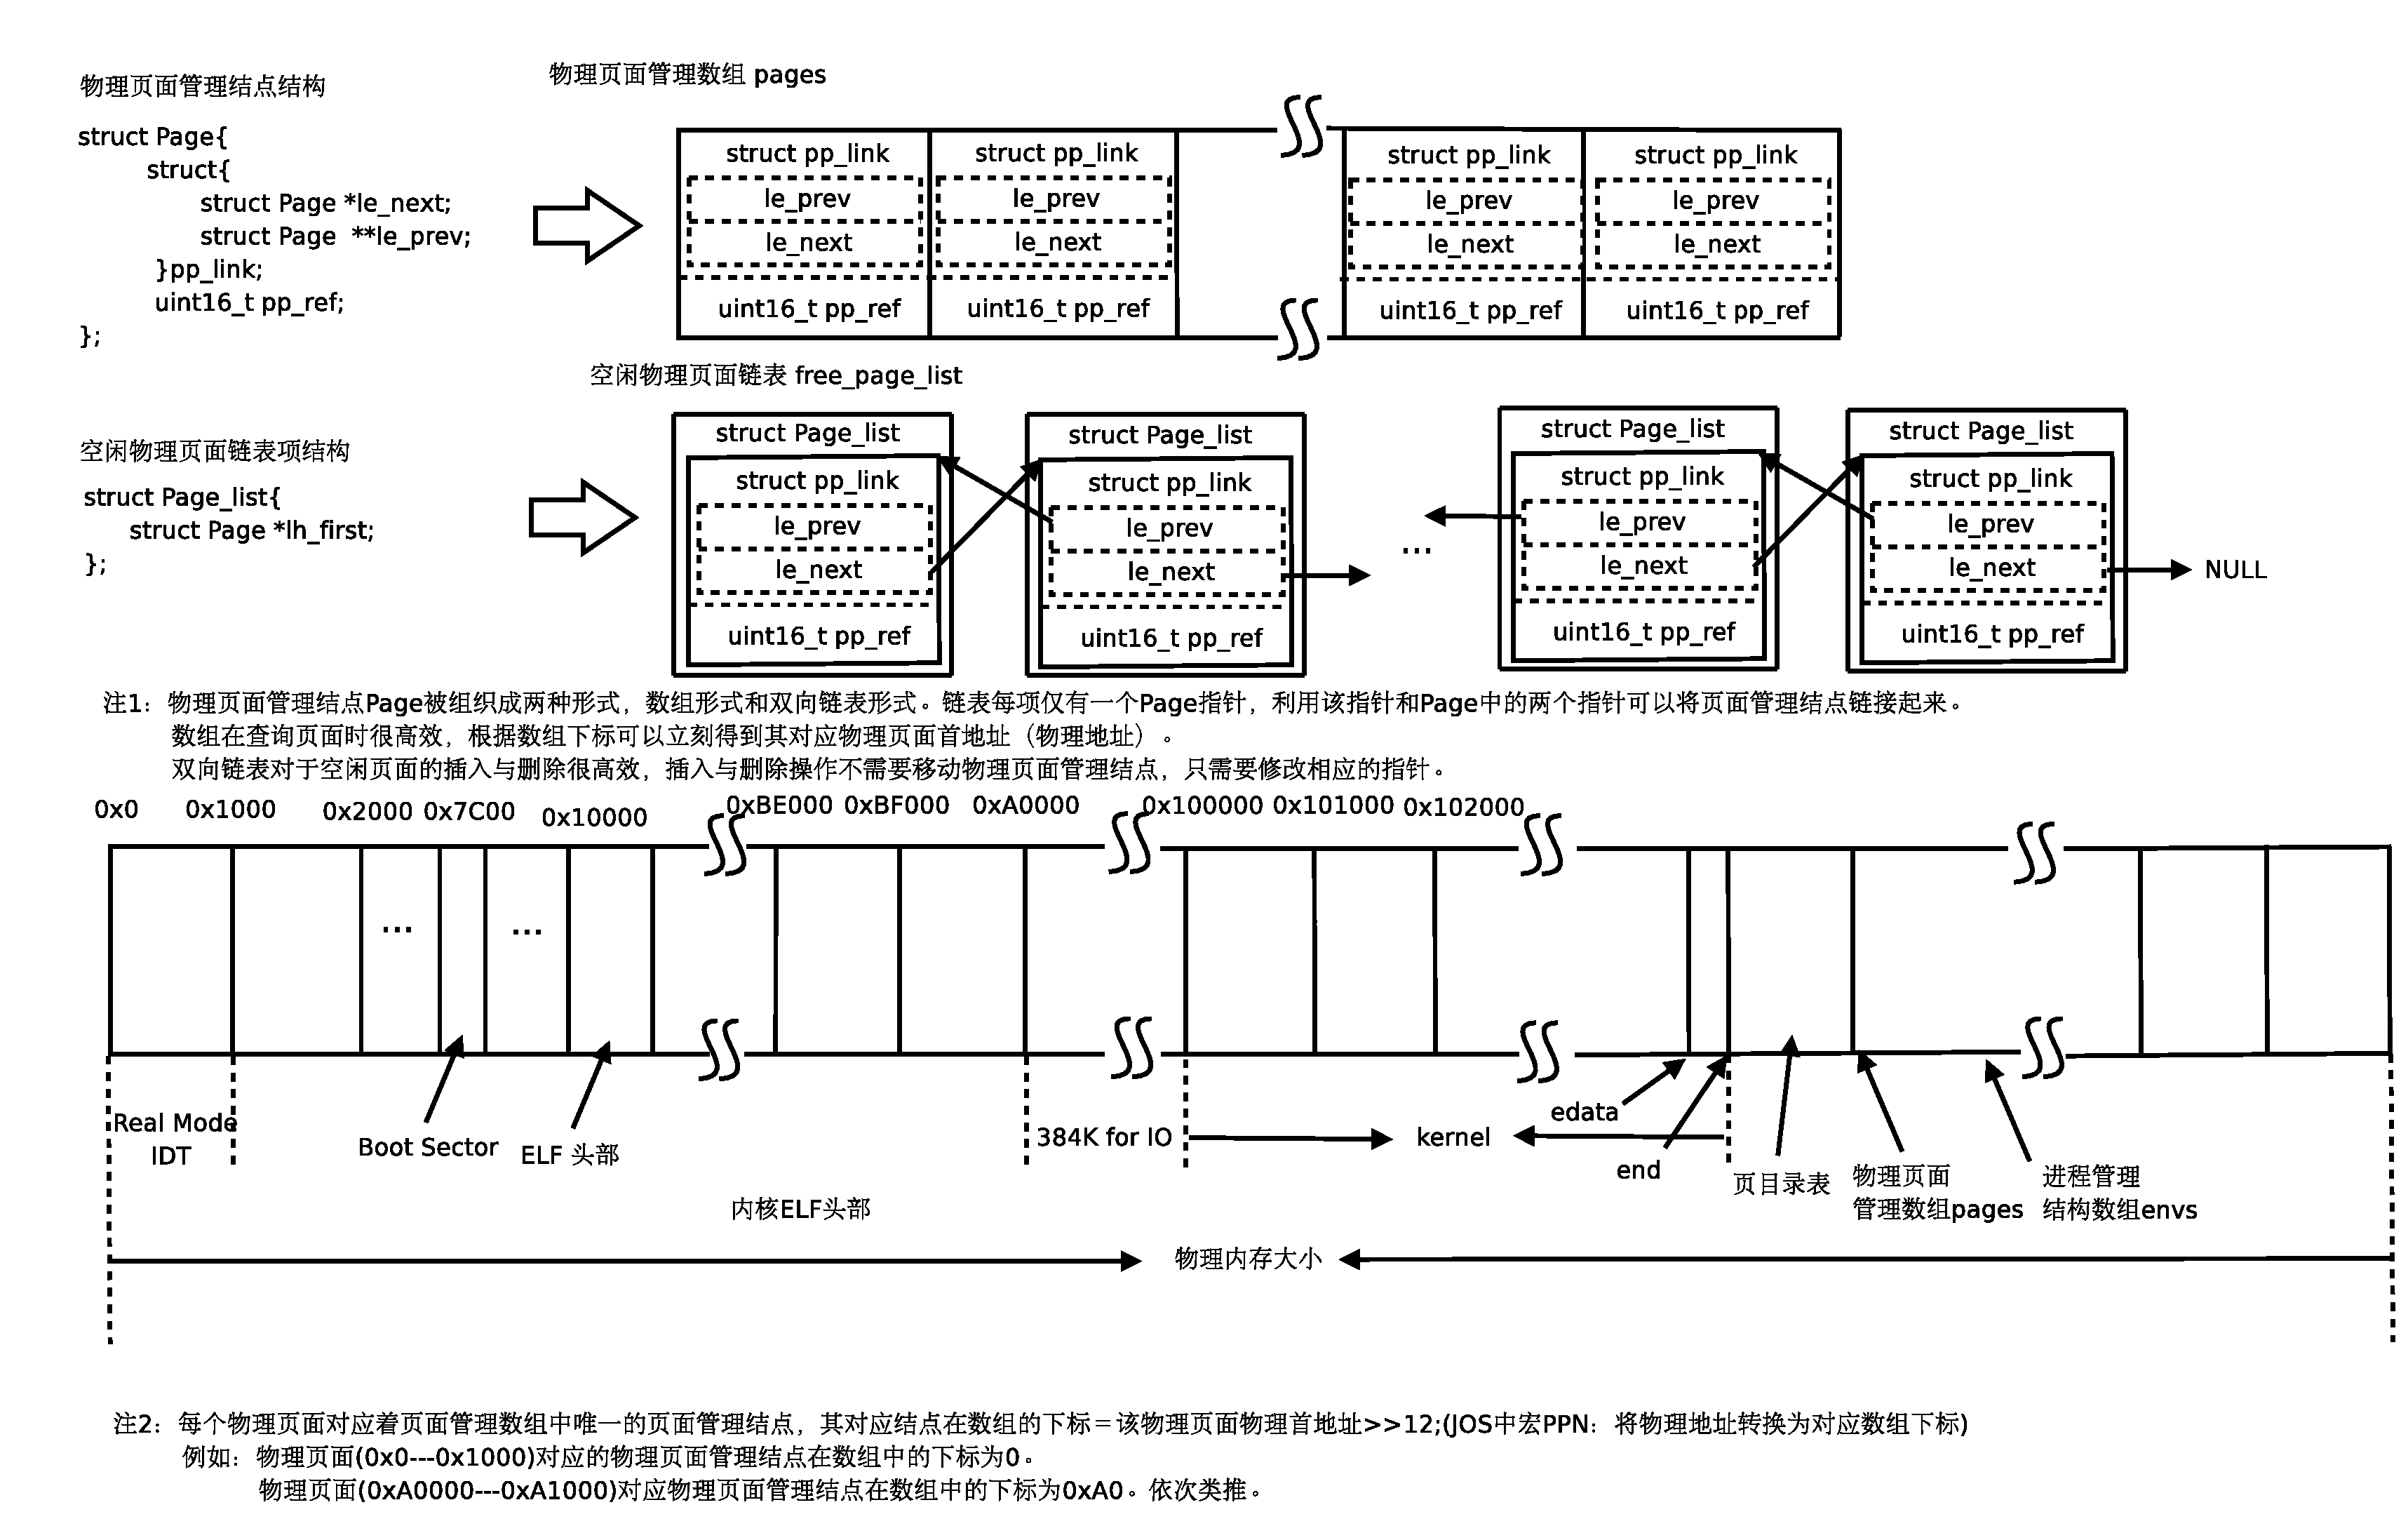
\includegraphics[height=10cm]{pages.eps}
		\caption[物理内存页面管理]{物理内存页面管理}
	\end{figure}

	    	\subsubsection{物理页面管理结构初始化}
	    物理页面管理部分提供了管理结点数组pages和空闲页面管理链表free\_page\_list的初始化函数
	page\_init,该函数为系统所有物理内存页面初始化唯一的页面管理结点,将系统正在使用的物理内存
	(如BIOS IDT占用内存,为IO操作预留的内存,内核代码占用内存,内核所用数据结构占用内存等)
	的引用标志为设置为1,其他空闲物理内存对应管理结点链入空闲物理页面链表中,
	并将其引用标志为设置为0。\par
	    	\subsubsection{分配一个物理页面}
	    在初始化物理页面管理结点和空闲物理页面链表之前,需要为内核几个重要的数据结构分配物理内存
	(如系统页目录表,页面管理结点数组和进程管理结点数组)。
	    JOS提供了分配一个物理页面的函数page\_alloc,该函数先检查空闲页面管理链表是否为空,不为空就
	从链表头摘下一个物理页面管理结点,并将该管理结点所有数据项情况。具体物理页面的清空操作和页面管理
	结点中引用标志的设置都不在该函数完成,由调用者操作。\par
	    	\subsubsection{释放一个物理页面}
	    物理页面释放功能通过page\_decref和page\_free两个函数完成。当要释放一个物理页面时,先调用
	page\_decref将该物理页面对应的管理结点中的引用标志减一,并检查其引用标志是否为0,如果为0,则
	调用page\_free将该页面管理结点插入到空闲物理页面链表中。\par	    

	\subsection{虚拟内存管理}

	    JOS中,开启分页之前,由于分段机制内核的虚拟地址和线性地址不同,还没有开启分页机制,所以
	线性地址和物理地址相同。JOS在开启分页机制时,同时将GDT表中的段基地址设置为0,这样虚拟地址和
	线性地址相同,相当于关闭分段机制,线性地址通过分页机制转换为物理地址。\par
	    由于JOS内核与用户程序共享4GB的虚拟内存空间,需要谨慎安排整个虚拟空间的布局,在根据布局
	建立虚拟内存与实际物理内存的映射关系。这样做的好处是当控制流从用户层陷入到内核层时,不需要
	切换cr3,也不需要刷新TLB,大大减少cache miss。\par
	    \subsubsection{JOS虚拟内存地址空间布局}
	    为内核预留固定虚拟地址空间,同时为用户层进程预留虚拟地址空间。需要隔离内核虚拟地址空间和
	进程虚拟地址空间,隔离不同进程虚拟地址空间。\par
	\begin{figure}[htb]
		\centering
		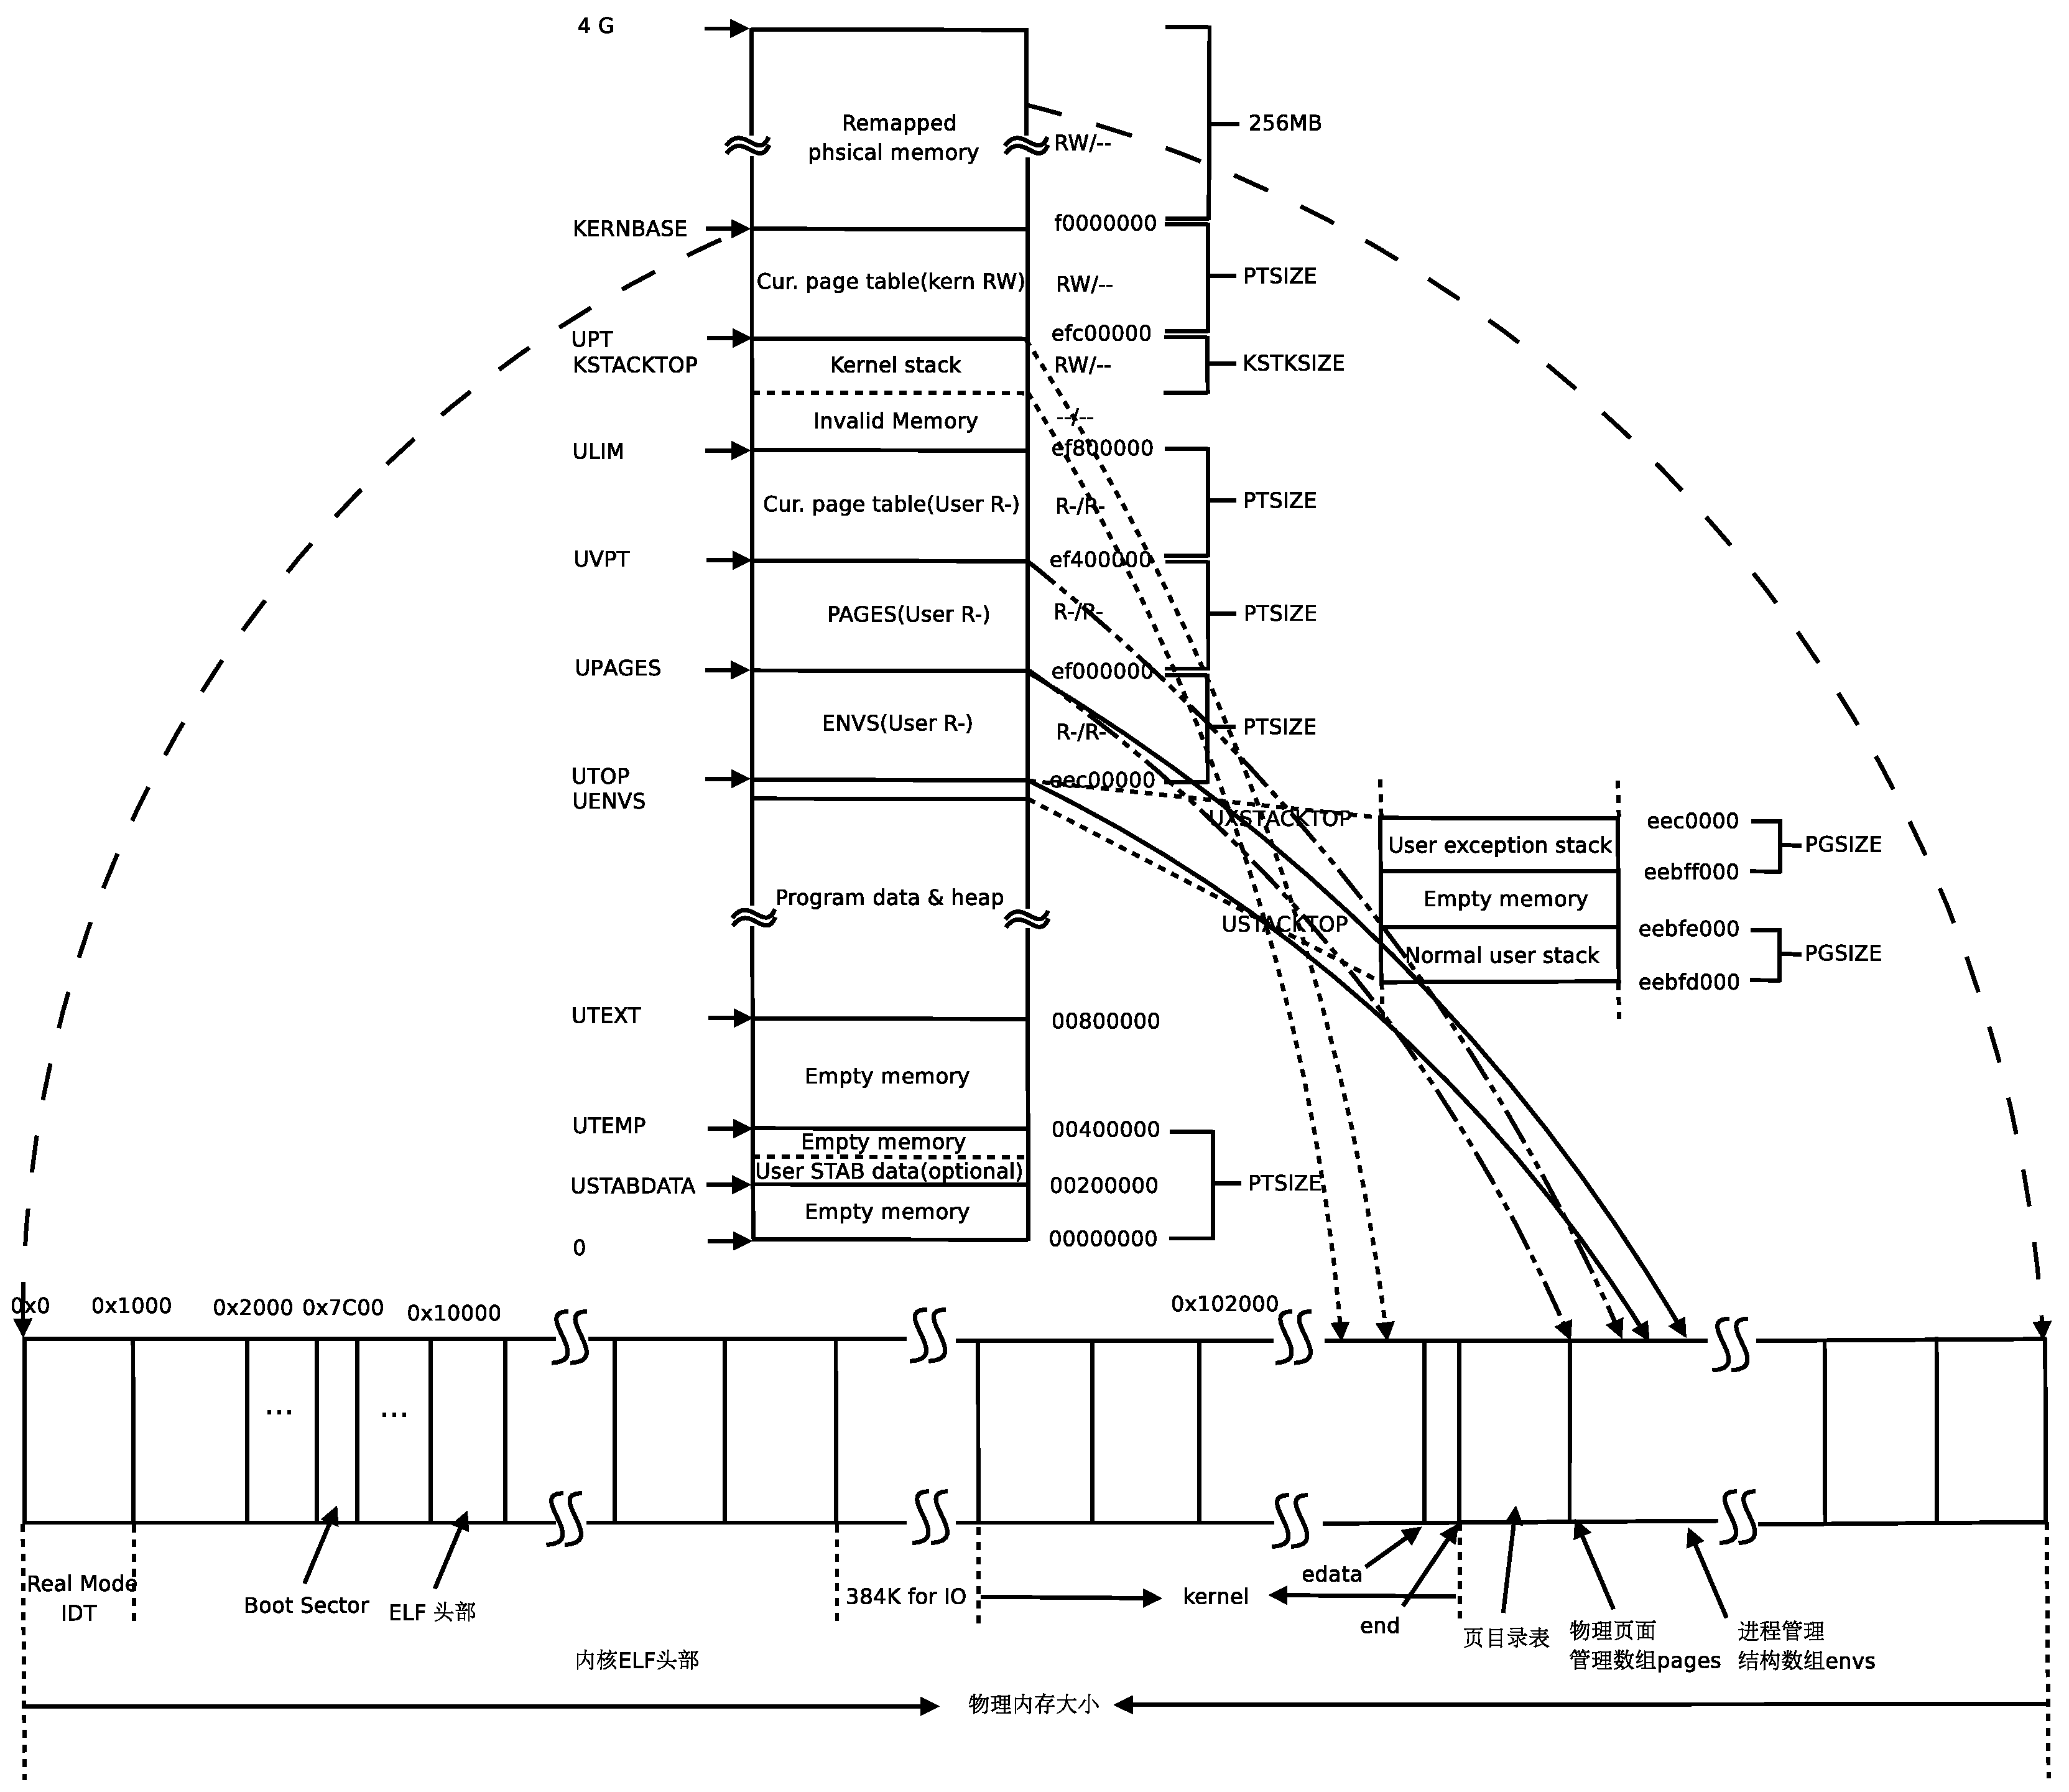
\includegraphics[height=12cm]{jos_layout.eps}
		\caption[虚拟内存空间布局]{虚拟内存空间布局}
	\end{figure}
	    在开启分页机制之前,JOS先设置内核虚拟地址空间的布局,也就是建立相应的页目录表和页表,
	建立相应虚拟地址到物理内存地址的映射关系。用户虚拟地址空间布局的相应页目录和页表建立在进程
	初始化阶段完成。\par
	    内核虚拟地址空间主要包括用于内核代码和数据的256M虚拟地址空间(0xf0000000--0xffffffff),
	用于当前页目录表和页表的所有项的4MB虚拟地址空间(0xefc00000--0xf0000000和0xef400000--0xef800000),
	用于内核栈的8个
	页面的虚拟内存地址空间(0xefbf8000--0xefc00000),栈顶虚拟地址是KSTACKTOP(0xefc00000)。
	同时内核还将当前使用的页表信息,页面管理结构信息,进程管理结构信息只读映射方式提供给
	用户层进程,但这些信息对于内核和用户都是只读的。其中页面管理结构信息和进程管理结构信息
	在内核的数据段。这样用户层的进程无须陷入内核态就可以访问这些重要信息,大大提高系统性能。
	还有一点需要注意的是,虚拟地址空间(0xef800000--0xefbf8000)是无效虚拟内存,内核和用户态都
	不能访问,这段虚拟内存地址可以作为内核栈的“保护页面”。\par
	    内核对内核当前使用页表和页目录表的映射进行了多次(3次)映射,第一次映射是与内核数据一起映射到
	高端地址(0xf0000000--0xffffffff),第二次映射以内核态读写权限映射到(0xefc00000--0xf0000000),第三次
	映射以用户态只读权限映射到(0xef400000--0xef800000),后两次映射操作有些特殊,下面详细介绍。\par
	
	\begin{figure}[htb]
		\centering
		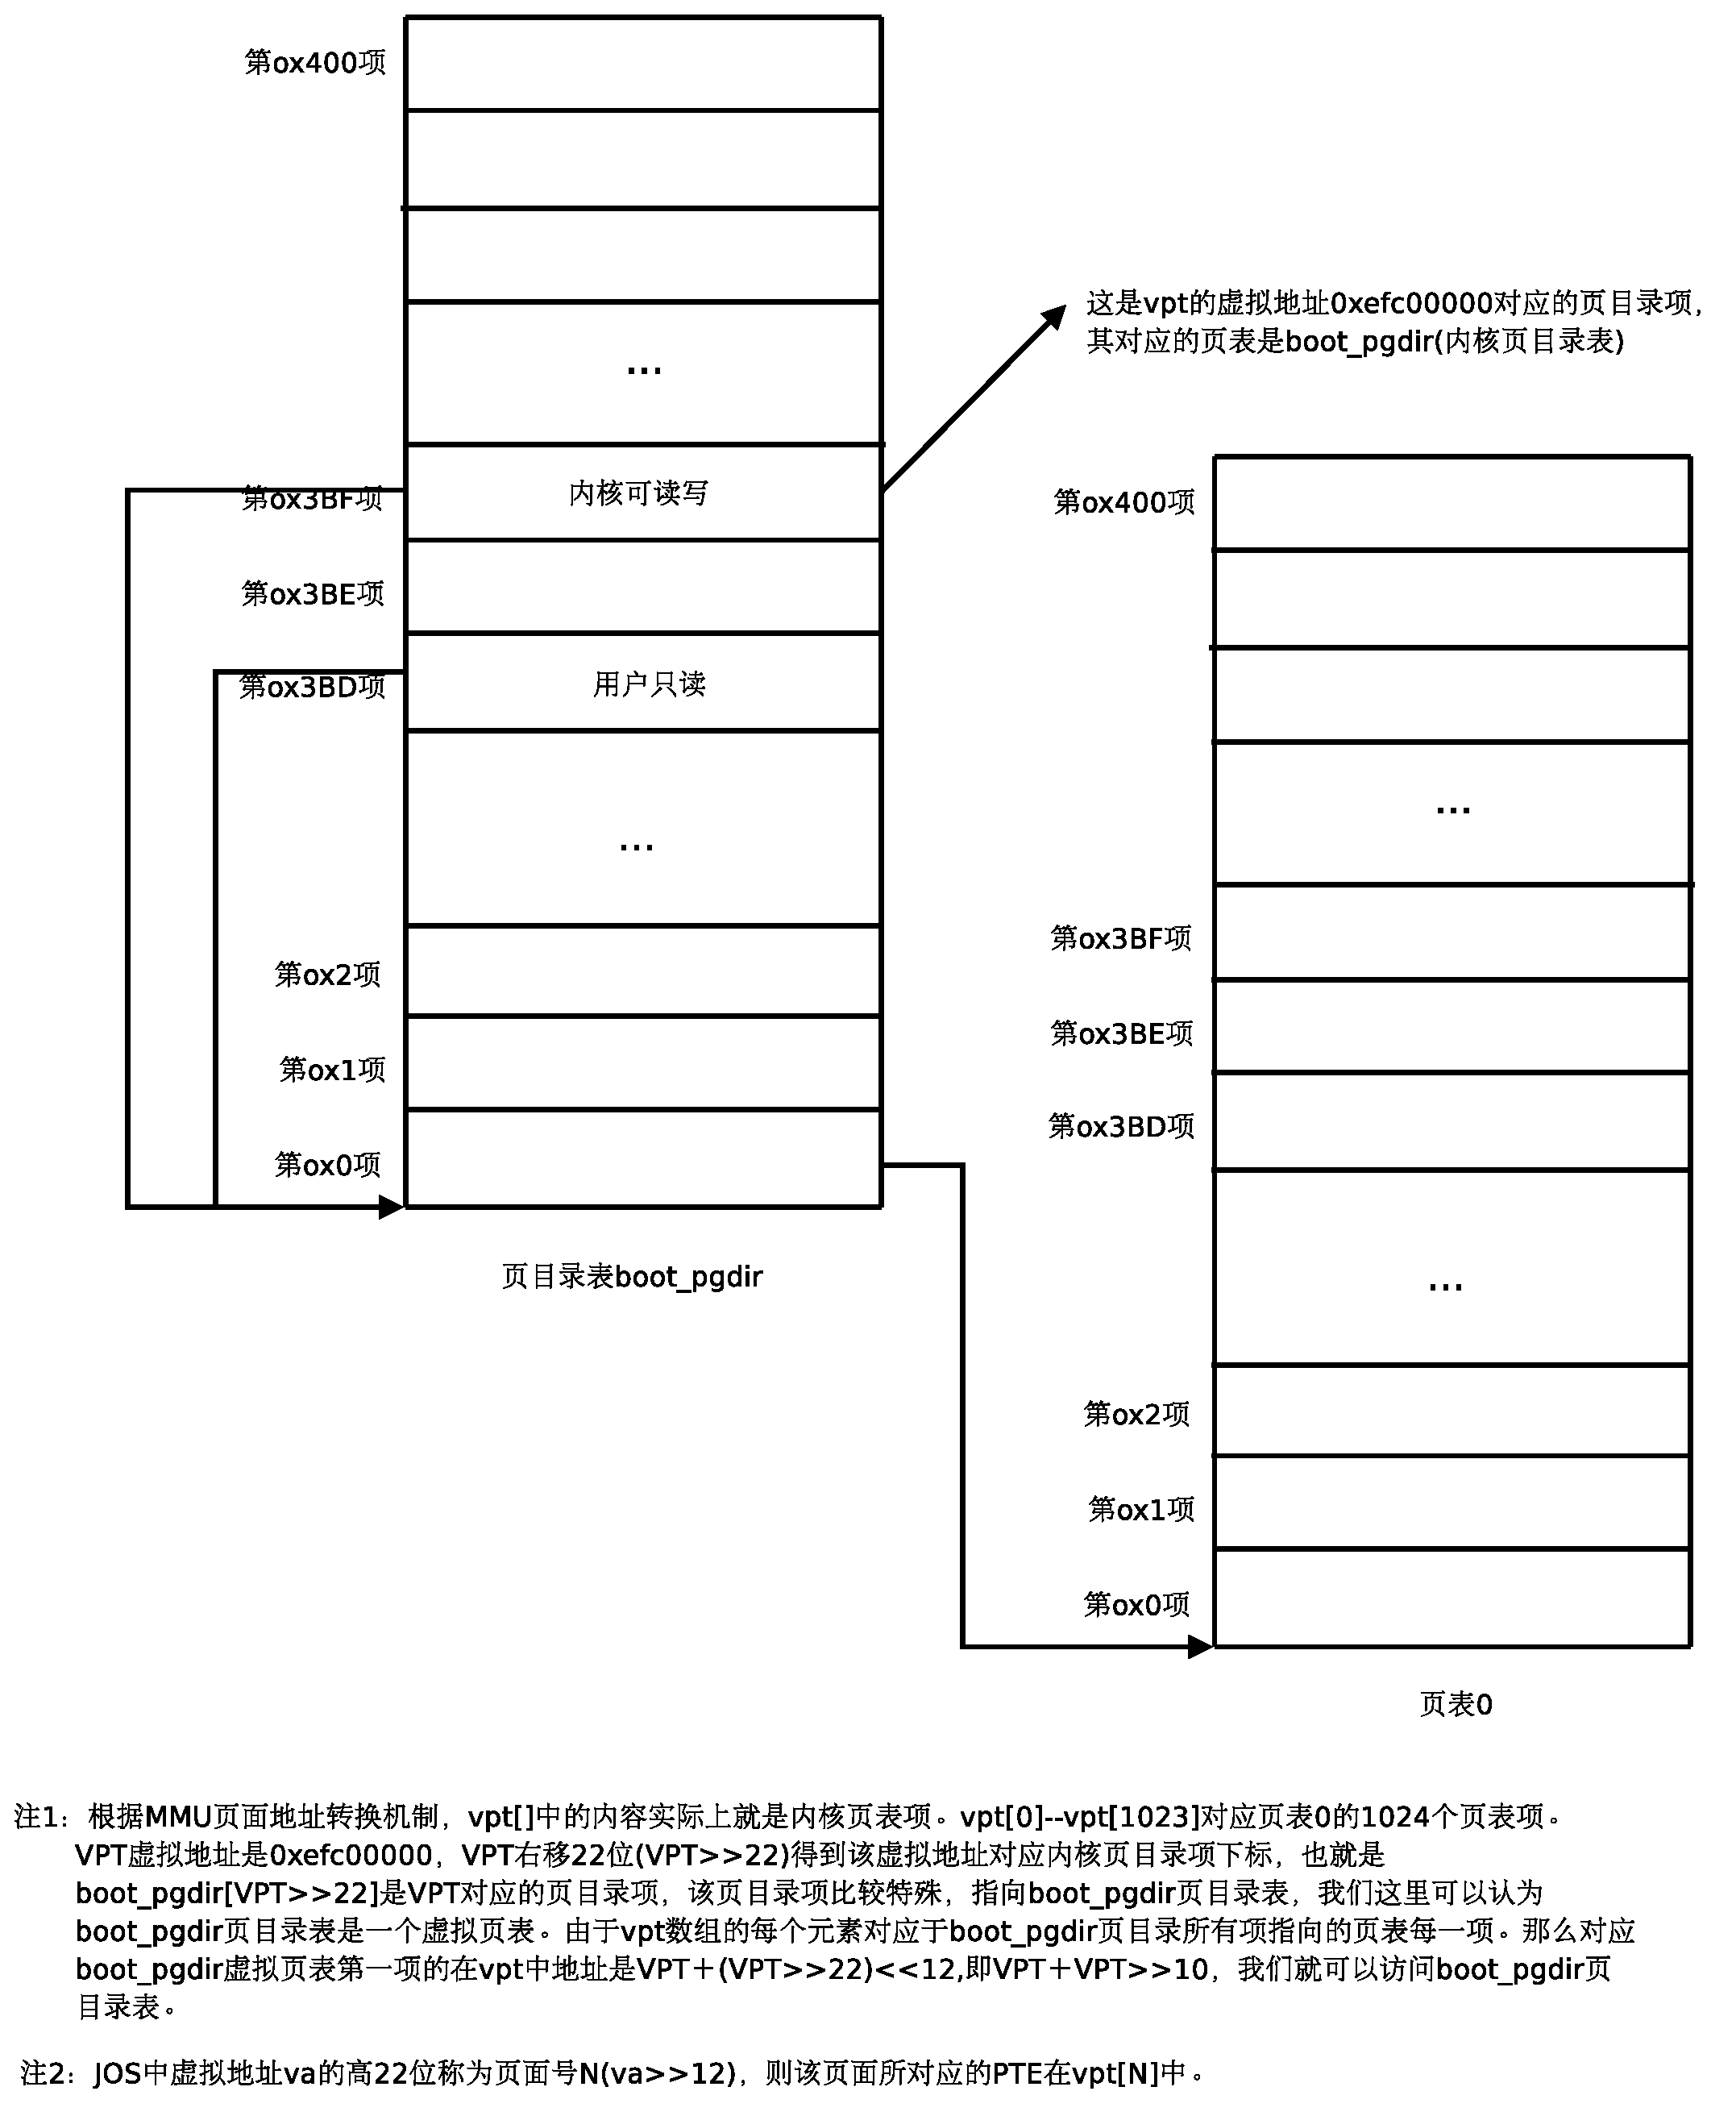
\includegraphics[height=12cm]{vpt.eps}
		\caption[内核页表和页目录共享映射]{内核页表和页目录共享映射}
	\end{figure}

	    在开启分页机制前,内核利用物理内存分配器boot\_alloc创建页面目录表boot\_pgdir,并根据虚拟
	内存地址空间布局完成相关映射。同时为了方便内核获取虚拟地址对应页表,JOS将内核页目录表boot\_pgdir
	和其目录项所指向的所有页表映射到虚拟地址(0xefc00000--0xf0000000)。采用的方法是找到虚拟地址
	(0xefc00000--0xefffffff)所对应页目录表boot\_pgdir所对应的页目录项,让该页面目录项指向页目录
	表boot\_pgdir,这时页目录表是一个虚拟页表(该页表中的每个项目是一个页目录项)。这样原来是内核页
	目录boot\_pgdir指向的所有页表(也包含了虚拟页表),现在成为了虚拟页表的对应的物理页面。
	在VPT(其值是0xefc00000)处定义一个页表项数组vpt,其下标是虚拟地址中的页面号
	通过vpt就可以访问修改内核创建的所有页表项和页目录项(页面目录项在虚拟页表中)。在$VPT+VPT\gg10$处定义
	一个页目录项数组vpt,其下标是虚拟地址中的页目录索引。同样的,将内核页表和页目录表的所有项以用户
	只读方式映射到UVPT。\par
	%%插入数学公式    
	%%\begin{displaymath}
	%%	VPT+VPT \gg 10
	%%\end{displaymath}
	
	    用户虚拟内存地址空间主要包括程序数据和堆的虚拟地址空间,普通用户栈虚拟地址空间,用户异常
	栈虚拟地址空间。具体虚拟地址空间布局和设计在后面章节详细介绍。\par
	    \subsubsection{内核虚拟地址空间}
	    JOS将处理器的32位线性地址空间分为两部分。用户环境(进程)将控制整个低部分的布局和内容,
	内核总是维护整个高部分的控制。内核预留大约256MB的线性地址空间。这解释了为什么我们需要给
	内核高链接地址(0xf0100000),否则,在内核的虚拟地址空间中没有足够的空间来同时进行用户环境
	中的映射。\par
	\subsubsection{基于分页机制的页面映射管理}
	\textbf{页目录和页表操作的核心函数}\par
	    JOS在内核中提供了页目录和页表操作的核心函数pgdir\_walk和page\_loopup。pgdir\_walk模拟
	x86分页硬件,查找与一个虚拟地址对应的页表项,该函数利用虚拟地址的高10位查找页目录项,页目录
	项的存在标志为0,相应页表页不存在。创建标志create,create为0表示当页表项不存在时,直接返回
	一个空值;为1表示当页表项不存在时,需要创建页表并修改填写相应页目录项,清空该页表的所有页表项。
	最后,利用虚拟地址的第二个10位可以找到页表项在页表页中的地址。\footnote{\tiny注意这里页目录项
	中的地址都需要填写物理地址,而访问页目录和页表用的地址,返回的页表项地址都是虚拟地址。}
	page\_loopup函数是查询映射到该虚拟地址的物理页面,主要用于页面释放page\_remove和验证页面权限。
	该函数返回物理页面管理结点和相应页表项,其主要过程是先利用pgdir\_walk查找虚拟地址对应的页表项,
	根据页表项中的物理地址可以得到相应物理页面管理结点。\par
	\textbf{页面映射}\par
	    page\_insert是JOS内核中页面支持最重要的一个函数,该函数的功能是将物理页面管理结点所对应
	的物理页映射到虚拟地址,填写相应页表项,修改物理页面管理结点中的引用标志位,刷新TLB。这里需要
	考虑虚拟地址已经指向了另外一个物理页面的情况,这时候需要调用page\_remove将该物理页面和虚拟地址
	的映射关系删除,再修改虚拟地址对应页表项。\par
	    boot\_map\_segment修改页目录表和页表创建从一段物理地址空间到相同大小的虚拟地址空间映射。
	在这个函数中需要检查重映射。该函数是一次映射一个页面,一直循环直到所有虚拟地址空间映射到相应物理地址
	空间,利用pgdir\_walk找到虚拟地址对应页表项,填写物理地址和访问权限。\par
	\textbf{页面映射撤销}\par
	    page\_remove是撤销虚拟地址与相应物理页面的映射关系。先利用page\_lookup找到虚拟地址所映射到的物理
	页面对应的物理页面管理结点和相应页表项。调用page\_decref修改物理页面管理结点,清空页表项,刷新TLB。
	如果虚拟地址没有被映射到任何物理页面,该函数不做什么。\par
	
	\section{进程管理系统设计与实现}
	    每个进程页表包含了用户内存和整个内核内存映射,这样由于系统调用或中断导致陷入内核,不需要
	切换页表。\par
	    在JOS内核中,对进程的管理和对物理内存页面管理相似,采用envs数组存储所有进程管理结点,利用
	数组下标可以快速索引某个进程管理结点,所有空闲的进程管理结点通过双向链表env\_free\_list进行管理
	    内核使用Env结构体来跟踪每个用户进程,进程管理结点是Env结构体定义的变量,
	JOS内核支持多进程。内核维护3个全局变量。envs是一个
	进程管理结构体Env的数组,系统中所有的进程都存放在这个数组里面。内核最多同时支持1024个活跃进程。
	内核初始化时候为envs数组分配空间,该数组有1024个进程结构体。JOS内核将所有非活跃进程结构体
	\footnote{\tiny非活跃进程结构体是指该进程结构体不指向任何进程,即该结构体是空闲可用的。}放入
	进程结构体空闲链表env\_free\_list中,该链表便于进程的分配与释放,仅仅需要从空闲链表中
	加入或删除一个结点。内核使用curenv变量时刻跟踪正在执行进程。在第一进程运行之前,curenv被设置为
	NULL。\par
	
		\begin{lstlisting}[language=C,numbers=left,numberstyle=\tiny,keywordstyle=\color{blue},frame=shadowbox,rulesepcolor=\color{red!20!green!20!blue!20},commentstyle=\color{red!50!green!50!blue!50!}\selectfont,basicstyle=\ttfamily\fontsize{8}{8}\selectfont]
/* kernel/env.c*/

struct Env *envs=NULL;		
struct Env *curenv=NULL;
static struct Env_list env_free_list;
		\end{lstlisting}
	\subsection{进程管理结构体}
	类似于Unix进程,JOS进程结合了线程和地址空间的概念,线程主要是通过被保存寄存器来定义
	(env\_tf字段),地址空间是通过页目录和页表来定义(env\_pgdir和env\_cr3)。在JOS中需要
	运行一个进程,内核必须使用进程管理结构体中的被保存寄存器和合适地址空间来设置处理器。
	内核在inc/env.h中定义进程管理结构体,具体如下图。\par
		\begin{lstlisting}[language=C,numbers=left,numberstyle=\tiny,keywordstyle=\color{blue},frame=shadowbox,rulesepcolor=\color{red!20!green!20!blue!20},commentstyle=\color{red!50!green!50!blue!50!}\selectfont,basicstyle=\ttfamily\fontsize{8}{8}\selectfont]
/* inc/env.h*/

struct Env{
	struct Trapframe env_tf;	//上下文记录
	LIST_ENTRY(Env) env_link;	//空闲链表链接指针
	envid_t env_id;			//唯一的进程标识
	envid_t env_parent_id;		//父进程的标识
	unsigned env_status;		//进程状态
	uint32_t env_runs;		//进程运行的次数
	
	//地址空间
	pde_t *env_pgdir;		//页目录表的内核虚拟地址
	physaddr_t env_cr3;		//页目录表的物理地址

	//异常处理句柄
	void *env_pgfault_upcall;	//页故障回调进入点

	//进程间通信
	bool env_ipc_recving;		//等待接收,进程阻塞
	void *env_ipc_dstva;		//将接收到的页面映射到该虚拟地址
	uint32_t env_ipc_value;		//发送的数据值
	envid_t env_ipc_from;		//发送者的进程标识
	int env_ipc_perm;		//接收到页面的映射权限
};

		\end{lstlisting}

	    结构体Trapframe用于保存寄存器状态,在inc/trap.h中定义。当用户进程不运行\footnote{\tiny在JOS中
	用户进程不运行是指处理器正在运行内核或其他进程。} 时,该结构体保存有关寄存器的值。当
	进程从用户态切换到内核态,由x86硬件或者内核将寄存器的值保存在结构体中(该结构体实际位于内核
	栈),从而进程可以从被中断的位置继续执行。结构体Trapframe是进程从用户态切换到内核态的关键
	数据结构。\par
	    进程结构体状态,空闲态表示该进程结构体是非活跃的,即该结构体不代表任何进程。可运行态表示
	该进程结构体是可运行的,即代表当前活跃进程,该进程处于就绪态。不可运行态表示进程结构体是不可运行的,
	即代表当前活跃进程,该进程处于阻塞状态。\par
	\subsection{进程创建}
	    在没开启文件系统服务之前,进程创建方法是JOS在内核态分配一个空闲的进程管理结点,并为该进程分配私有
	页目录表,将内核映射到其虚拟地址空间,并按上一章的JOS虚拟空间布局安排进程用户层虚拟地址空间。
	在内核编译链接中\footnote{\tiny用户程序的二进制镜像在obj/user/目录中,链接这些镜像时,使用
	了-b binary选项,将这些二进制镜像做为一个不可解释的二进制文件,作为一个整体嵌入到内核中,
	而不是常规.o文件。},内核将用户程序\footnote{\tiny这里的用户程序
	是指处于用户层的操作系统服务,例如文件系统服务,网络服务等。} 的静态二进制镜像以ELF可执行镜像嵌入
	在内核镜像中。在初始化进程管理结点和虚拟地址空间后,将用户程序镜像载入\footnote{\tiny链接器在将用户
	程序二进制镜像链接到内核时,在符号表中,编译器为每个镜像生成3个符号:\_binary\_obj\_user\_xxx\_start,
	\_binary\_obj\_user\_xxx\_end,\_binary\_obj\_user\_xxx\_size。内核代码可以利用这些符号来访问用户二
	进制镜像。}相应物理地址空间,并建立相关映射。用eip寄存器保存该用户程序镜像的入口地址。\par
	
	    进程创建主要分为两步:一是为该进程分配虚拟地址空间和空闲进程管理结点;二是将用户态程序的二进制
	镜像加载到内存中,并设置程序入口点。详细过程分为以下几个步骤:\par	
	    
	    (1) 分配一个空闲的进程管理结点并对相关字段进行初始化。从进程管理结点空闲链表中获取一个空闲结点。
	根据分配给进程的页目录表,初始化页目录表物理地址字段env\_cr3和页目录表虚拟地址字段env\_pgdir。根据
	该管理结点在全局数组的位置,为其生成一个唯一的进程标识env\_id。JOS内核态创建的进程是一类特殊
	的进程,提供传统操作系统内核的一些服务,如文件系统服务,网络系统服务,这些进程在内核初始化时创建
	并启动运行,因此内核定义它们没有父进程,其父进程标识字段env\_parent\_id为0。进程运行状态字段env\_status
	初始化为ENV\_RUNNABLE,表示该进程处于就绪态。进程的运行次数字段env\_runs初始化为0。为了防止前一个进程
	的信息泄露,需要先清空空闲进程管理结点的上下文记录子段env\_tf,再进行初始化,使用全局描述符表GDT已经
	定义好的用户数据段GD\_UD初始化数据段寄存器(ds,es)和栈寄存器(ss),用代码段GD\_UT代码段寄存器cs,
	初始化栈指针esp。指令指针eip应该初始化为进程的第一条指令,此时程序的二进制镜像还没有装载到内存中,故
	无法确定eip。为了在用户态接收中断,需要设置EFLAGS中的中断使能IF标志。清空页故障处理句柄字段
	env\_pgfault\_upcall,该句柄由用户程序使用相应系统调用设置。清空IPC接收标志字段env\_ipc\_recving。
	JOS默认将进程管理结点全局数组的第二个结点env[1]设置为文件系统服务进程管理结点,为了让文件系统服务
	进程能访问I/O地址空间,需要设置EFLAGS中的I/O特权级IOPL为3。清空该结点的空闲链表链接指针字段,
	将该结点移出空闲链表。\par
	
	    (2) 用户进程虚拟地址空间初始化分两步进行。用户进程虚拟地址空间布局主要包括内核部分(UTOP--4G)
	\footnote{\tiny内核代码和内核数据,内核栈,内核提供给用户的其他信息使用这部分虚拟内存}
	和用户部分(0--UTOP)\footnote{\tiny用户程序代码,用户数据,用户栈,用户程序的调试信息使用这部分
	虚拟内存}。内核和用户程序共享4G虚拟地址空间,在进程控制流从用户态转移到内核态时,不需要切换页
	目录,减少TLB刷新。使用内核物理页面分配函数page\_alloc每个进程分配一个物理页面作为其页目录表。
	内核部分对应的页目录项可以直接从内核页目录表boot\_pgdir直接拷贝过来。将进程所有页表映射到VPT,提供
	给内核使用,权限设置为可读写,同时将进程所有页面映射到UVPT,提供给用户进程使用,权限设置为用户态
	只读。用户部分的虚拟地址空间在用户程序链接时给代码段,数据段,调试信息段分配相应虚拟地址空间,
	用户程序二进制镜像ELF装载到物理内存时,将相应段映射到对应虚拟地址空间。\par
	    (3) 装载二进制镜像。利用编译器生成的符号\_binary\_obj\_user\_xxx\_start来引用xxx应用程序的
	二进制镜像。在链接脚本中设置应用程序代码段和数据段从虚拟地址0x800020处开始放置,设置调试信息
	STAB从虚拟地址0x200000处开始放置。采用segment\_alloc分配一定长度的物理内存给应用进程,并将它
	映射到进程地址空间相应位置。在应用程序的二进制镜像的头部字段e\_entry是程序入口虚拟地址,将
	该值赋给进程的eip字段。另外需要分配进程用户态栈,即分配一个物理页面,并映射到USTACKTOP-PGSIZE处,
	权限设置为用户态可读写,并初始化该物理页面。\par
	
	\subsection{进程调度}
	    JOS进程管理结点数组envs第一项是空闲进程,当系统没有其他待运行进程时,运行该进程。\par 
	    JOS内核采用时间片轮转算法选择下一个待运行进程管理结点,使用env\_run启动该进程。
	如果当前进程管理结点指针curenv不为NULL,就从进程管理结点数组envs中当前运行进程后面选择
	一个待运行的进程;当curenv为NULL时,从数组envs中的第二项开始查询,选择一个遇到的待运行
	进程。\par
	\subsection{进程销毁}
	     JOS内核中用env\_destroy来销毁一个指定进程。基本过程是释放该进程所有使用的物理页面(包括页目录表
	和页表),将进程管理结点字段env\_status赋值为ENV\_FREE,并将该结点插入空间进程管理结点env\_free\_list,
	如果要销毁的是当前进程,释放页面前需要将页目录表切换到内核专用的页目录表boot\_cr3,页面释放完成后,
	需要将当前进程指针赋为NULL,并调用sched\_yield调度下一个待运行的进程。\par


	\subsection{中断与异常}
	    中断和异常都是“受保护的控制转移”,将使处理器从用户态转移到内核态。为了确保这些受保护的控制转移
	是真正被保护的,处理器的中断或异常机制必须限制发生中断或异常时正在执行的代码转移到内核的入口点,
	以及进入内核的方式。处理器为了保证在受控条件下进入内核。使用了中断描述符表和任务状态段两种机制
	来提供保护。\par
	    中断发生在程序执行的随机时刻,以响应硬件发出的信号。系统硬件使用中断来处理外部事件,例如要求
	为外部设备提供服务。软件可以通过执行INT n指令产生中断。异常发生在处理器执行一条指令时,检测到一个
	出错条件时发生,例如被0除出错条件。处理器可以检测到各种出错条件,包括违反保护机制,页错误和
	机器内部错误等。\par
	    在JOS系统中,为了简化内核设计,进入内核立即关闭中断\footnote{\tiny目前JOS内核不支持抢占,
	有兴趣的读者可以改进内核,支持内核抢占},用户态进程态进程利用中断或异常与内核进行交互,
	如陷入内核,使用硬件资源。\par
	\paragraph{中断描述符表}
	    处理器确保中断和异常陷入内核的入口点是一些特定的并定义好的,内核自身
	确定入口点,中断和异常发生时正在运行的代码不能决定入口点。x86允许最多256个不同中断或异常内核入口点,
	每个入口点由一个唯一中断向量号标识。中断向量号是0至256之间的一个数。一个中断的向量号由中断源决定,
	对于不同设备,错误条件和应用向内核的请求有不同向量号。CPU使用向量号作为处理器中断描述符表的索引,
	类似于GDT内核在自身私有地址空间建立该表。x86处理器执行指令时检测到的同步异常使用中断向量号
	0至31,对应于IDT表中的0-31项。通过INT指令产生的软件中断或异步硬件中断使用的中断向量号大于31。\par
	    IDT表中可以存放三种类型的门描述符号,分别是中断门描述符,陷阱门描述符和任务门描述符。JOS系统中,仅仅
	使用了中断门和陷阱门,它们含有一个长指针(即段选择符和偏移量),处理器使用这个长指针把程序控制权转移到
	内核中断或异常处理入口点。这两个门唯一区别在于处理器操作EFLAGS寄存器IF标志上。当通过中断门访问一个
	异常或中断处理过程时,处理器会复位IF标志以防止其他中断干扰当前中断处理过程。随后的IRET指令会用保存在
	内核栈上的内容恢复EFLAGS寄存器的IF标志。通过陷阱门访问处理过程并不会影响IF标志。\par

	\paragraph{任务状态段}
	    在处理中断或异常前,处理器需要将被中断或发生异常程序状态保存在内核栈中,
	如调用异常处理程序之前的EIP和CS寄存器值,这样异常处理程序在处理完后能恢复处理器状态,继续执行被中断代码。
	必须保护保存处理器状态的内核栈,防止非特权用户态代码访问。当x86处理器利用中断或异常实现从用户态到
	内核态的转换,同时进行栈的切换\footnote{\tiny用户态栈切换到内核栈}。任务状态段(TSS)指定了内核栈的
	堆栈段寄存器SS和堆栈指针ESP。栈切换下面详细介绍。\par
	    在控制从用户态转移到内核态,处理器从当前执行任务TSS段\footnote{\tiny在JOS系统中,内核和用户进程使用同
	一个任务状态段,不发生任务的切换,任务状态段主要是在中断或异常时,提供内核栈}中得到中断或异常处理过程
	使用的堆栈的段描述符SS和栈指针ESP。处理器通过硬件自动将被中断程序的SS,
	ESP,EFLAGS,CS,EIP和一个可选错误码压入刚切换的内核栈中。硬件自动使用对应中断描述符信息设置CS和EIP,
	设置ESP和SS指向内核态栈。\par
	    在JOS系统中,仅仅使用了TSS中的栈信息来定义内核栈,当处理器从用户态切换到用户态时,处理器利用该信息
	进行栈切换。JOS中的内核运行在x86特权级0,使用TSS中的ESP0和SS0定义内核态栈。\par
	\paragraph{中断和异常使用的主要数据结构}
	    JOS中使用结构体Trapframe保存上下文,这主要有以下两个目的:中断处理程序根据中断号tf\_trapno和错误码
	tf\_err进行相应处理;中断处理完成后,恢复上下文,将控制权从内核态转移到用户态,被中断应用程序继续执行。
	Trapframe中与硬件自动压入栈相关寄存器\footnote{\tiny如SS,ESP,EFLAGS,CS,EIP,
	错误码(可选)}对应字段顺序应该和它们在栈中顺序保持一致。其他字段顺序和相关代码一致。\par

	    JOS中使用pushal指令在中断发生时统一保存通用寄存器的值;在返回被中断程序时,使用popal指令
	恢复通用寄存器的值。结构体PushRegs中各字段顺序与这些寄存器值在栈中顺序一致\footnote{\tiny这里的一致是
	表示第一个字段是最后入栈的寄存器,在栈中的顺序可以参考Intel手册}。\par
		\begin{lstlisting}[language=C,numbers=left,numberstyle=\tiny,keywordstyle=\color{blue},frame=shadowbox,rulesepcolor=\color{red!20!green!20!blue!20},commentstyle=\color{red!50!green!50!blue!50!}\selectfont,basicstyle=\ttfamily\fontsize{8}{8}\selectfont]
/* inc/trap.h*/
struct Trapframe {//最后入栈的在低地址,最先入栈的在高地址
        struct PushRegs tf_regs;
        uint16_t tf_es;
        uint16_t tf_padding1;
        uint16_t tf_ds;
        uint16_t tf_padding2;
        uint32_t tf_trapno;  //中断号
        /* below here defined by x86 hardware */
	//发生中断时,下面寄存器内容由硬件将其自动压入栈中
        uint32_t tf_err;    
        uintptr_t tf_eip;
        uint16_t tf_cs;
        uint16_t tf_padding3;
        uint32_t tf_eflags;
        /* below here only when crossing rings, such as from user to kernel */
        uintptr_t tf_esp;
        uint16_t tf_ss;
        uint16_t tf_padding4;
} __attribute__((packed));
		\end{lstlisting}

		\begin{lstlisting}[language=C,numbers=left,numberstyle=\tiny,keywordstyle=\color{blue},frame=shadowbox,rulesepcolor=\color{red!20!green!20!blue!20},commentstyle=\color{red!50!green!50!blue!50!}\selectfont,basicstyle=\ttfamily\fontsize{8}{8}\selectfont]
/*inc/trap.h*/
struct PushRegs {
        /* registers as pushed by pusha */
        uint32_t reg_edi;
        uint32_t reg_esi;
        uint32_t reg_ebp;
        uint32_t reg_oesp;              /* Useless */
        uint32_t reg_ebx;
        uint32_t reg_edx;
        uint32_t reg_ecx;
        uint32_t reg_eax;
} __attribute__((packed));
		\end{lstlisting}
	\paragraph{中断向量表的初始化}
	    中断向量表IDT初始化主要包括初始化IDT中门描述符,定义并实现各个中断对应的中断处理函数。
	定义各个中断处理过程在内核中的入口地址对应函数名,即中断向量号为N的中断处理函数名为vectorN。
	定义一个存放各个中断处理函数首地址的全局数组vectors,向量号为i的中断对应中断处理函数
	首地址存放在与数组第i项。利用perl脚本生成vectors.S给数组赋值。利用宏为每个中断生成中断处理函数。
	使用全局数组vectors的信息初始化对应的IDT中的门描述符。在JOS中,仅仅使用了中断门,在用户程序被
	中断时,处理器自动复位EFLAGS中的IF标志,从而实现在内核中关闭中断,从内核态返回用户态时,
	处理器自动设置EFLAGS中的IF标志,开启中断。在内核中关闭中断主要是为了简化设计和安全性考虑。\par
	\paragraph{中断和异常的处理流程}
	    在JOS系统中,中断和异常的处理由软硬件协同完成。处理器硬件主要检测中断或异常信号;从TSS
	中获得内核态栈的段地址SS0和栈顶指针ESP0;将被中断程序的SS,ESP,EFLAGS,CS,EIP的值压入
	内核栈中;用户态栈切换到内核态栈,SS和ESP指向内核态栈;根据处理器产生的中断向量号和IDTR寄存器
	中的基地址,查找IDT表中对应门描述符,将门描述符中的段描述符赋给CS,过程入口点偏移赋给EIP,控制
	从用户程序转移到内核中断处理入口点。\par
	
	\begin{figure}[htb]
		\centering
		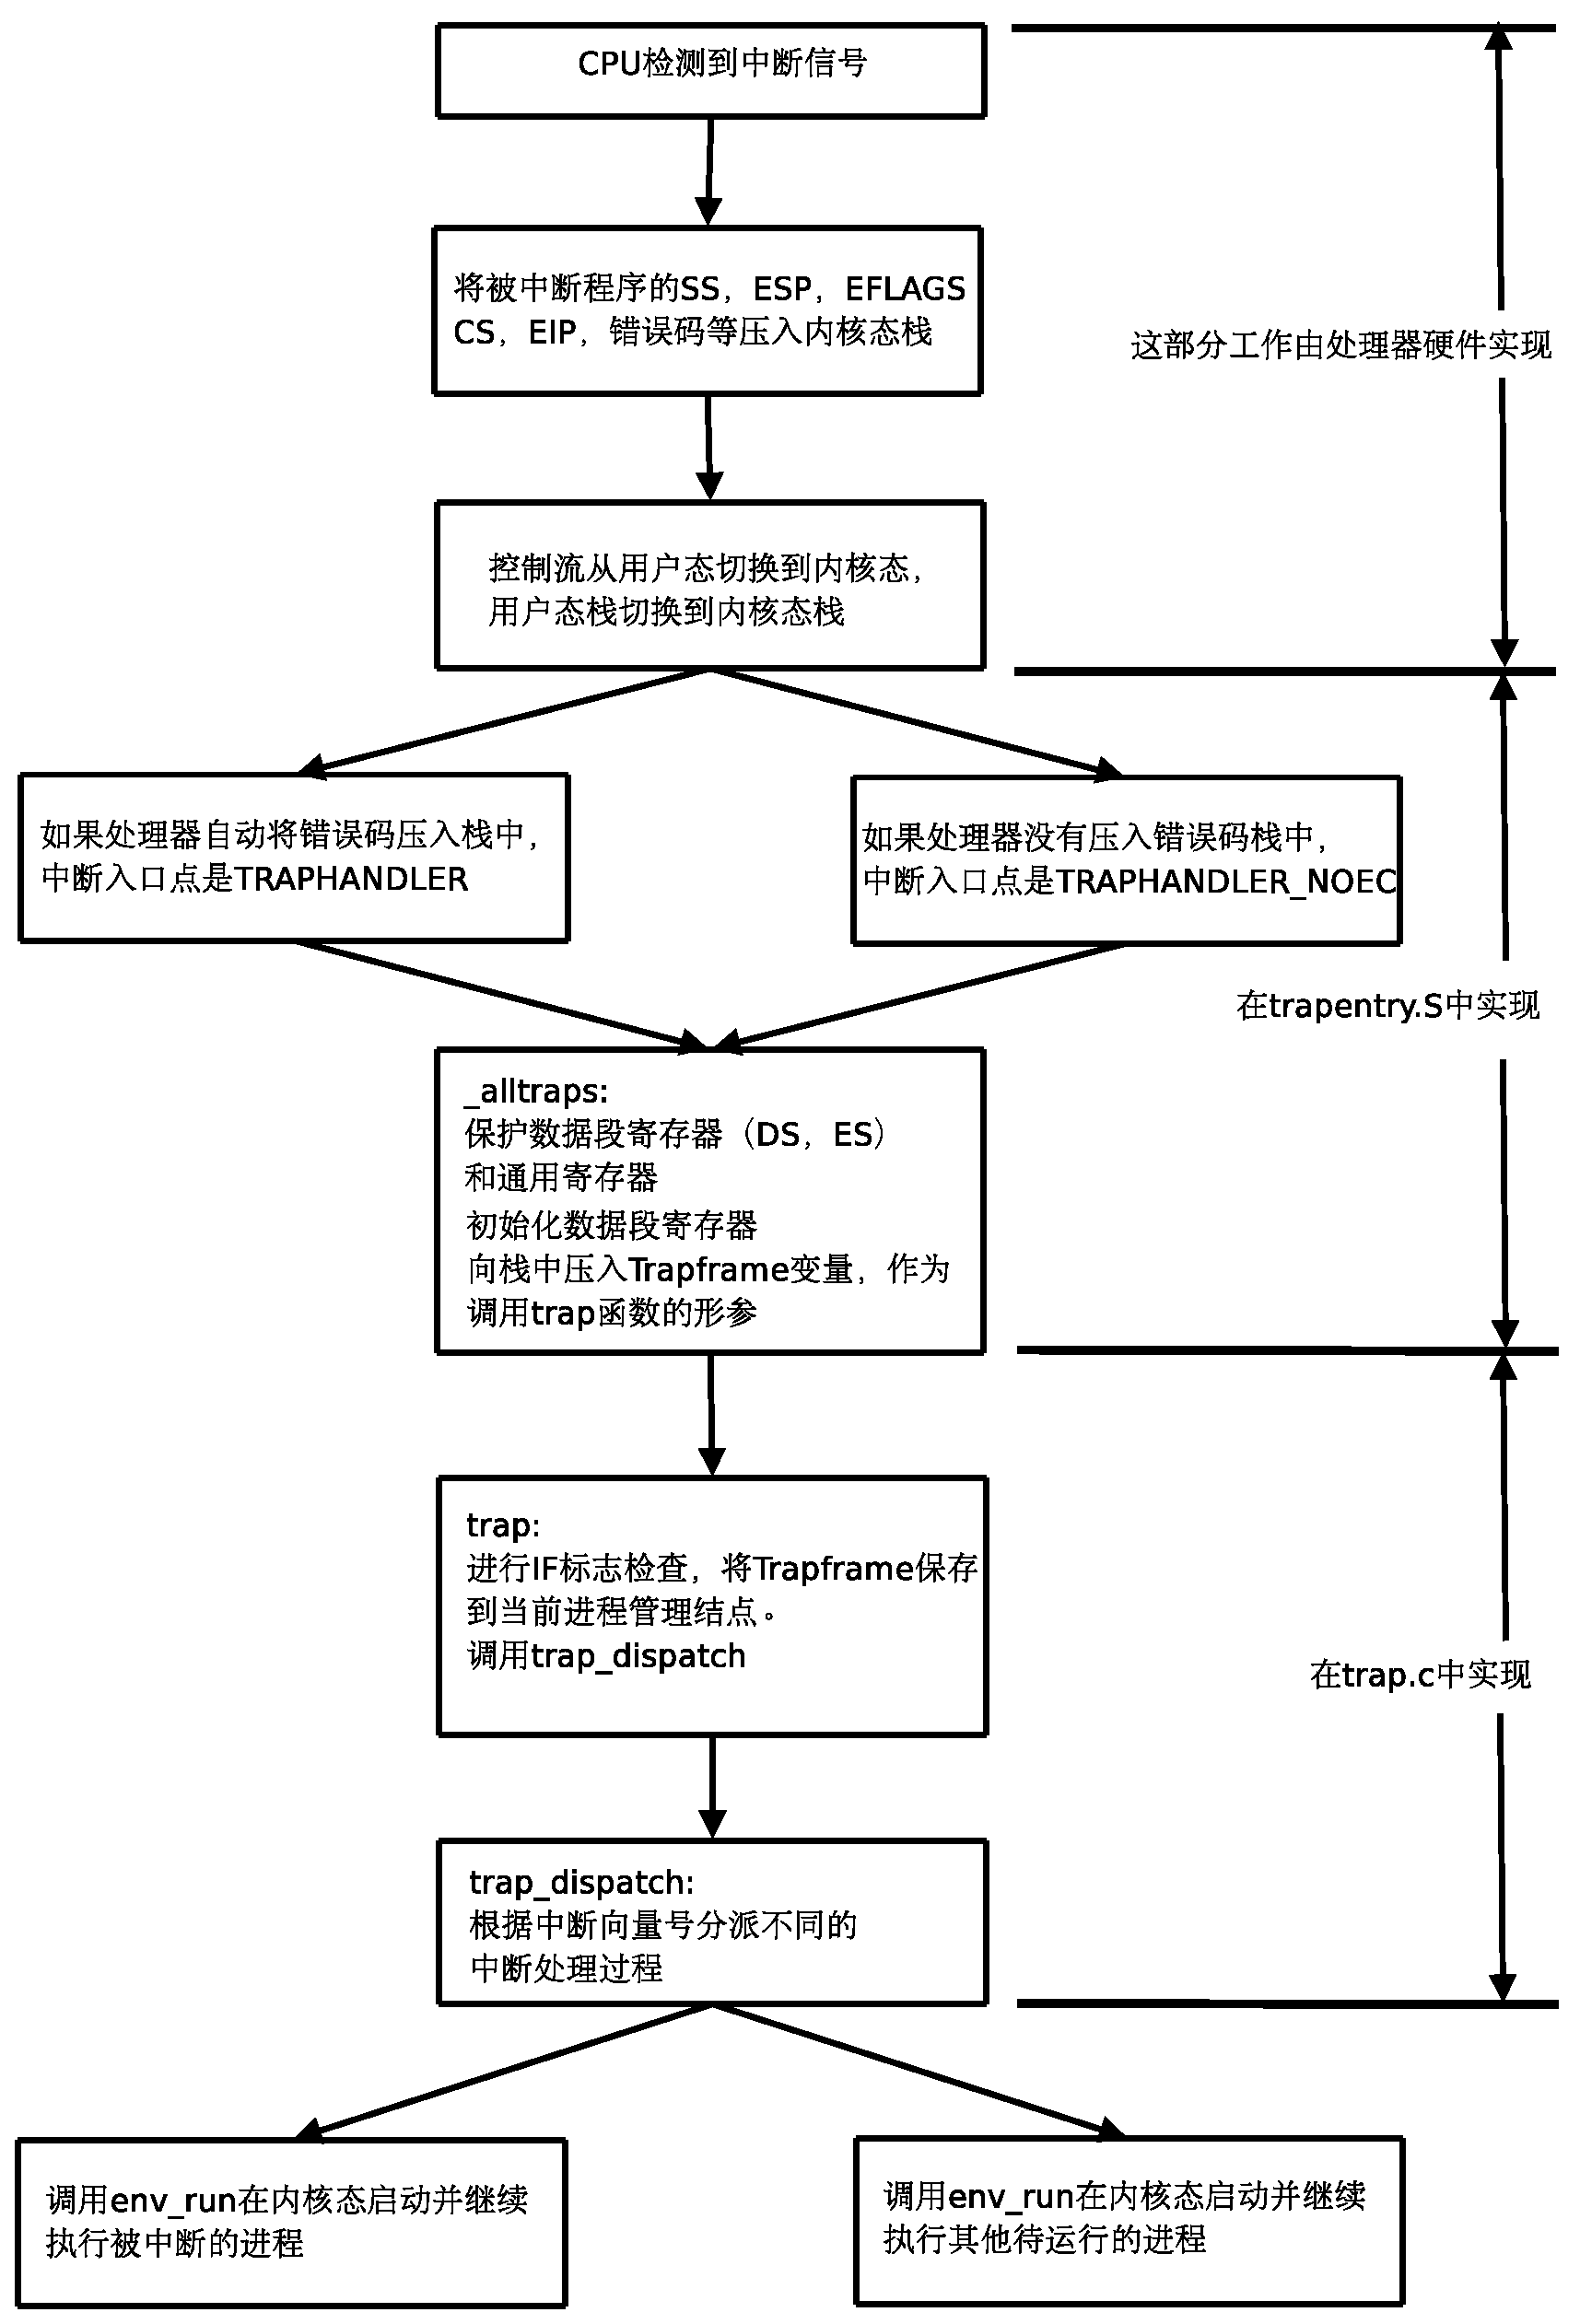
\includegraphics[height=12cm]{interrupt.eps}
		\caption[中断和异常的处理流程]{中断和异常的处理流程}
	\end{figure}

	    所有中断处理程序都需要保护上下文,合法性检查。在JOS中对所有中断被真正处理之前,将上下文统一
	保存栈中,形成一个Trapframe类型的变量,并检查处理器是否自动复位EFLAGS中的IF位。将栈中保存的上下
	文存储在当前进程管理结点env\_tf字段。根据进程管理点记录的中断向量号,调用不同的中断处理过程。
	中断处理过程结束后,内核调用env\_run继续运行刚被中断的进程,但在中断处理处理过程中内核会调用
	env\_run启动另一个进程来处理中断。特殊的是时钟中断发生,表示当前进程的时间片耗尽,系统挂起
	该进程,启动下一个进程\footnote{\tiny这里描述的是时间片轮转算法,但并不表示JOS只能采取该
	调度算法,这里主要是说明中断在进程切换中的作用}。\par  

	\subsection{上下文切换}
	    上下文切换是指程序从一种状态切换到另外一种状态(例如从内核态切换到用户态),或从一个程序切换到
	另一个程序(例如进程切换)时,导致上下文相关寄存器值的变化行为。JOS系统中,进程切换的基本过程是
	一个进程通过中断机制陷入到内核,内核将该进程的上下文保存在内存(进程管理结点)中,内核按一定调度
	策略选择下一个要运行的进程管理结点。\par   
	    JOS系统中,将操作系统大多数功能作为一个用户态进程运行,在进程创建完成后,由内核完成
	从内核态到用户态的切换,启动用户态进程,所采用的方法是模拟中断调用返回过程,即利用iret指令来实现
	特权级的变更和栈的切换,从而把CPU执行控制流转移到用户态进程中\footnote{\tiny这里eflags里面的NT标志为0,
	表示CPU执行iret指令不会导致任务的切换。},详细过程如下。\par
	    在从内核态切换到用户态之前,当前运行进程指针curenv指向将要切换到的
	进程对应管理结点,管理结点的进程运行次数记录项env\_runs加1,内核为用户进程设置虚拟地址空间,
	即切换到进程管理结点中的env\_cr3所指向的页目录。利用进程管理结点中的env\_tf保存信息初始化
	通用寄存器\footnote{\tiny通用寄存器包括edi,esi,ebp,ebx,edx,ecx,eax,用指令popal/pushal将这些
	寄存器的值出/入栈。},段寄存器\footnote{\tiny段寄存器主要有ds,es,cs,ss等}。
	设置内核堆栈,模拟具有特权层切换的刚进入中断调用过程时栈内容布置情况如下图所示。执行iret指令,x86
	硬件会自动顺序将内核栈中的EIP,CS,EFLAGS,ESP,SS寄存器值弹出到相应寄存器中。\par
	
	\begin{figure}[htb]
		\centering
		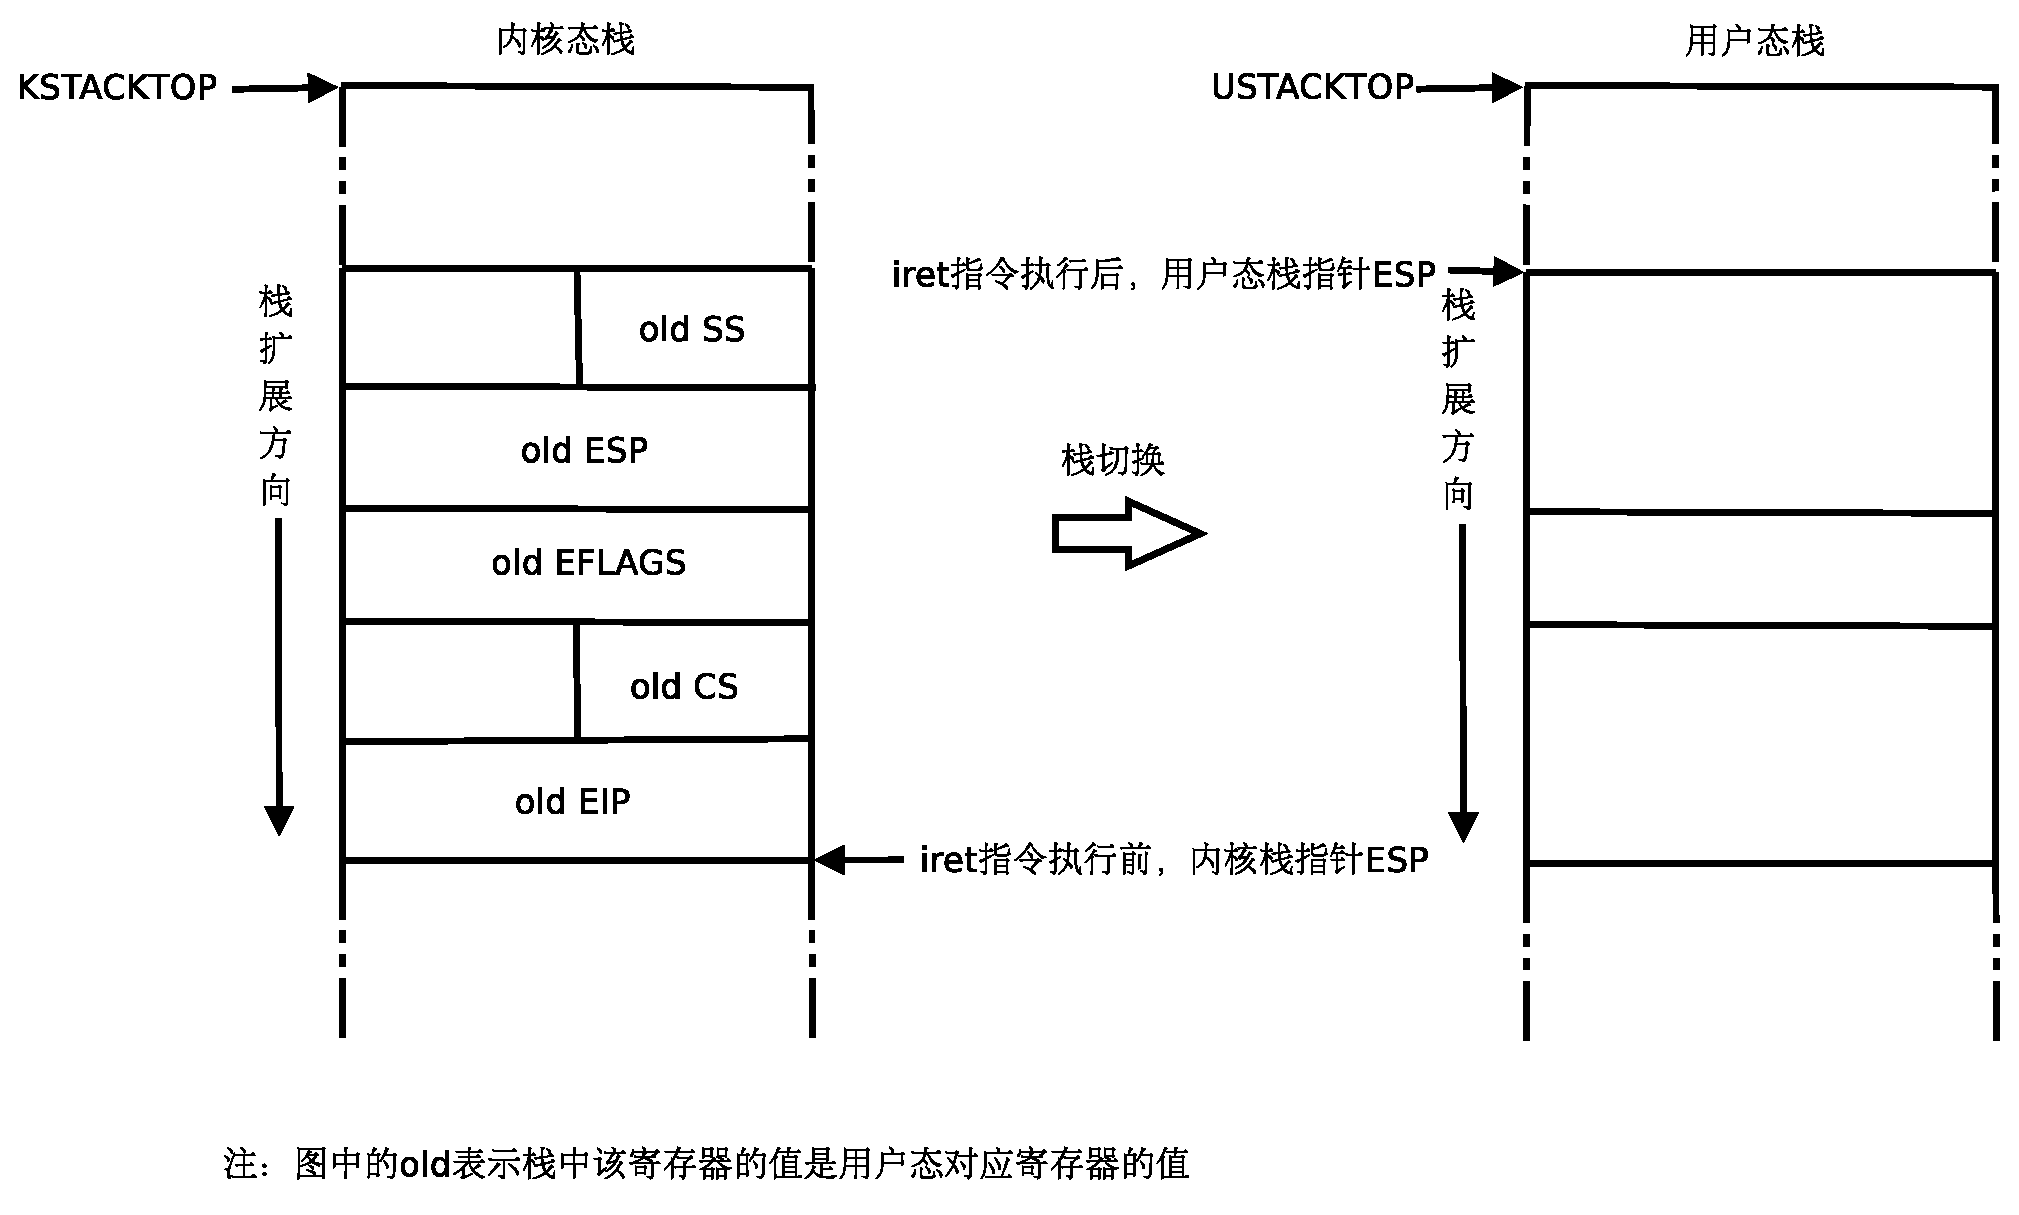
\includegraphics[height=8cm]{iret.eps}
		\caption[内核态栈到用户态栈切换]{内核态栈到用户态栈切换}
	\end{figure}
	
	    从用户态切换到内核态主要是通过中断处理完成了,详细过程参考上一小节“中断与异常”。\par
	\subsection{基于异常处理的操作系统原语}
	    利用软硬件中断和异常处理机制可以构建页故障处理,断点异常处理和系统调用等重要
	操作系统原语。\par
	\paragraph{1 页故障处理}
	    
	    内存保护是操作系统的关键特性,确保一个程序中的bugs不会使其他程序崩溃或操作系统自身
	崩溃。操作系统通常依靠硬件支持来实现内存保护。操作系统保证硬件知道那些虚拟地址是有效的,
	那些是无效的。当程序试图访问一个无效地址或没有权限访问,处理器将使程序停在引起故障的指令
	处,再陷入到内核。如果故障是可修复的,内核修复它,程序继续运行。如果故障是不可修复的,
	程序不能继续运行。\par
	    系统调用给内存保护引入了一个有趣的问题。大部分系统调用接口允许用户程序传递指针到
	内核。这些指针指向用户可读写的缓冲。内核执行系统调用时解引用这些指针。这将引发两个问题:\par
	
	    1. 内核中页故障比用户程序中页故障更具有潜在危害。如果内核在操作自身数据结构时发生页
	故障,这是一个内核bug,页处理程序应用冻结内核。但当内核解引用用户程序提供的指针时,这
	需要方法记住由这些解引用操作引起的任何页故障是用户程序的页故障。\par
	    2. 内核通常比用户程序有更多权限。用户程序可能传递一个指针给系统调用,内核能读写该指针指向的内存,
	但用户程序可能没有写权限。为了防止泄露私有信息或不、破坏整个内核完整性,内核不能解引用该指针。\par
	    解决上面两个问题的方法是内核仔细检查所有从用户空间传递到内核的指针。当一个用户程序向内核传递
	一个指针,内核将检查地址是否是地址空间用户部分,页表是否允许内存操作。\par
	
	\paragraph{(1) 触发页面故障的条件}
	    页面故障异常对应的中断向量号是14。当开启页面机制,即控制寄存器CR0中的PG为1,处理器在将线性地址
	转换为物理地址时检测到下列条件之一将触发页面故障异常:\par
	    1. 在地址转换中相应页目录项或页表项中的存在位为0。\par
	    2. 当前过程没有访问特定页面的足够权限\footnote{\tiny例如写一个只读页面(COW技术)}。  \par
	    处理器硬件自动将错误码压入栈中,引起页面故障的线性地址保存在控制寄存器CR2中,页面故障处理程序
	可以利用这两个信息诊断和修复页面故障。\par
	\paragraph{(2) 用户级页面故障处理机制}
	    JOS中用户进程在普通执行过程使用普通用户栈。栈指针指向USTACKTOP。当页故障发生在用户模式,进程陷入
	内核态,JOS内核重新启动进程运行已分配好的用户级页面故障处理程序,使用用户异常栈在普通执行过程使用普通
	用户栈。栈指针指向USTACKTOP。当页故障发生在用户模式,进程陷入内核态,JOS内核重新启动进程运行已分配好
	的用户级页面故障处理程序,使用用户异常栈。JOS内核为用户进程进行自动“栈切换”,所采用的方法类似于
	x86处理器为JOS在控制由用户态转移到内核态时进行栈切换。\par
	    JOS用户异常栈的大小是一个页面。栈顶是UXSTACKTOP。当用户进程使用这个异常栈时,用户级页故障处理
	程序可以使用JOS常规的系统调用来映射新页面或调整映射来修复页故障引发的问题。用户级页故障处理
	程序通过一个汇编语言程序返回到引起页故障的代码,使用原来用户普通栈。\par
	    popal指令将edi,esi,ebp,ebx,edx,ecx,eax分别出栈,不将esp出栈。\par
	\paragraph{用户级页面故障处理程序注册}
	    在用户级定义页面故障处理程序,该处理函数统一为输入是结构体struct UTrapframe的指针,无输出。
	并在用户态程序中调用set\_pgfault\_handler向JOS内核注册该处理程序。JOS在用户级使用sys\_page\_alloc
	为进程分配一个用户态可读写物理页面,并将该页面映射到UXSTACKTOP-PGSIZE处;向进程管理结点注册一个
	页面故障处理统一入口点\_pgfault\_upcall,用全局函数指针\_pgfault\_handler保存用户自定义的
	页面故障处理程序入口地址。整个注册工作都在JOS用户态完成。\par
	\begin{figure}[htb]
		\centering
		\includegraphics[height=10cm]{pgfault.png}
		\caption[用户自定义页面故障处理过程注册]{用户自定义页面故障处理过程注册}
	\end{figure}

	\paragraph{用户级页面故障处理基本过程}
	    
	\paragraph{2 断点异常处理}
	    断点异常对应的中断向量号是3。调试器使用int 3软中断指令在程序代码中插入一个断点。JOS
	中将断点异常作为一个基本伪系统调用,任一用户进程都可以使用该异常来调用JOS内核监视器。
	内核监视器是一个基本的调试器,断点异常的方法是合适的。例如,用户态panic函数在显示
	了进程当前上下文信息,再执行int 3指令。\par
	\paragraph{3 系统调用}
	    用户进程通过系统调用获取内核服务。当用户程序调用一个系统调用,先进入内核态,处理器
	和内核协同保存用户进程状态,内核执行相应代码完成系统调用,再继续执行用户进程。\par
	    在JOS内核中,我们使用int指令引发一个系统调用。使用int \$0x30作为系统调用中断。需要
	在全局描述符数组idt设置对应中断描述符,让用户进程产生该中断。并在trap\_dispatch中根据
	中断向量号调用kern/syscall.c中syscall函数进行处理,syscall函数是所有系统调用的入口点。\par	
	    应用程序使用寄存器传递系统调用号和系统调度参数。这样内核不需要访问用户进程栈或指令
	流。系统调用号保存在eax寄存器中,5个参数分别保存在edx,ecx,ebx,edi,esi寄存器中,内核
	将系统调用返回值保存在eax寄存器中。\par

	\section{多任务设计与实现}

	\section{文件系统设计与实现}

	\paragraph{文件系统原语}
	   目前实现的文件系统比现实中的文件系统更简单,但也具有基本功能:创建文件,
	读文件,写文件,和删除文件,以层次化目录结构组织文件。\par
	\paragraph{磁盘文件系统结构}
	   大多UNIX文件系统把可用磁盘空间分成两种主要区域:inode区和数据区。UNIX文件系统
	给文件系统中每个文件分配一个inode;文件的inode包含文件的关键元数据,如属性stat和
	指向其数据块的指针。数据区被划分为多个数据块(通常8KB或更大),在文件系统中,
	这些数据块存储文件数据和目录元数据。\par	
			\subsubsection{网络驱动设计与实现}

	\section{JOS技术创新点}
	这是另一个小节。
		\subsection{系统初始化}
			\subsubsection{技术点分析}
		\subsection{内存管理}
	  %% \begin{figure} ... \end{figure} 这部分的内容并做相应修改
	        \subsection{用户环境} 
	        \subsection{多任务}
	        \subsection{文件系统}
	        \subsection{网络驱动}

	\section{JOS研究与发展}
		\subsection{MIT研究进展及技术贡献}
		\subsection{其他相关研究}
%%------------ 参考文献  -------------%%
%\bibliographystyle{plain}
%\addcontentsline{toc}{chapter}{参考文献}
%\phantomsection
\addcontentsline{toc}{chapter}{参考文献}
\begin{thebibliography}{99}
	%Linux起源(历史)、发行版介绍
    	%\bibitem{prefone}文献条目1, 作者, 期刊 刊号, 年份
	%Linux特点(相对于Windows/Unix/Solaris)
	%\bibitem{preftwo}文献条目2, 作者, 书名, 年份
	%贡献者介
	%\bibitem{prefthree}文献条目3, 作者, 书名, 年份
	%内核整体视图
	%\bibitem{preffour}文献条目4, 作者, 书名, 年份

	%系统初始化
	%内存管理
	\bibitem{Extensibility} Dawson R. Engler, M. Frans Kaashoek, and James W. o'Toole Jr. The exokernel approach to extensibility.In 1st OSDI, Nov, 1994.
	\bibitem{Exokernel} D.R.Engler, M.F.Kaashock, and J.o'Toole. Exokernel:An operating system architecture for application-level resource management.In 15th SOSP,Dec, 1995.
	\bibitem{AppFlexibility} M.Frans Kaashoek, Dawson R. Engler, Gregory R. Ganger etc. Application Performance and Flexibility on Exokernel Systems. In 16th SOSP, Oct, 1997.
	\bibitem{AppNetworing} Gregory R. Ganger, Dawson R. Engler, M. Frans Kaashoek etc. Fast and Flexible Application-Level Networking on Exokernel Systems. ACM Transaction on Computer Systems. 2002, 20(1):49-83.
	\bibitem{Exo04} Tim Leschke. Achieving Speed and Flexibility by Separating Management from Protection:Embracing the Exokernel Operating System. Operating Sytems Review. 2004,38(4):5-19
	\bibitem{Underware} D Irwin, Jeff Chase, Laura Grit, Aydan Yumerefendi, and Jeannie Albrecht. Underware:An Exokenel for the Internet?. 2007.
	\bibitem{Corey} Sialas Boyd-Wickizer, Haibo Chen, Rong Chen, Yandong Mao etc.Corey:An Operating System for Many Cores.In 8th OSDI. Oct.2008.
	\bibitem{Determinitor} Amittai Aviram,Shu-Chun Weng,Sen Hu, Bryan Ford. Efficient System-Enforced Deterministic Parallelism. In 9th OSDI. Oct.2010.
	\bibitem{XOmB} J. Larkby Lahet, B.A. Madden, D. Wilkinson, and D. Mosse. XOmB:an exokernel for modern 64-bit,multicore hardware. In WSO-VII Workshop de Sistemas Operacionais. July, 2010.
	\bibitem{LKD}wolfgang Mauerer, 深入理解linux内核架构, 2012,6
	\bibitem{LK}DANIEL p.BOVET ,MARCO CESATI, 深入理解 LINUX 内核,第3版
	\bibitem{LVM}Understanding the Linux Virtual Memory Manager.pdf
	\bibitem{CSS}Randal E.Bryant David R.O'Hallaron, 深入理解计算机系统, 2011,1
	\bibitem{MOS}Andrew S. Tanenbaum ,现代操作系统,第3版  2009,7
	\bibitem{MM}关于linux内存管理, http://blog.csdn.net/macrocrazier/article/details/6705298
	\bibitem{Xen}辛晓慧,Xen内存虚拟化实现---影子页表内存管理机制  
	%用户环境
	%多任务
	%文件系统
	%网络驱动
	%相关研究
\end{thebibliography}
%%------------- 正文结束 --------------%%

%%-------------- 以下是附录 ---------------%%	
\begin{appendix}
\chapter{附录标题1}
	\section{附录1.1}
\end{appendix}
\end{document}
